% Template for Elsevier
% version 1.1-5p dated 18 January 2011
% NO ACCENTUATION PROBLEM UTF-8 : NOT ACCEPTED

% This file (c) 2010-2011 Elsevier Ltd. Modifications may be freely made,
% provided the edited file is saved under a different name

% This file contains modifications for Procedia Computer Science
% but may easily be adapted to other journals


%-----------------------------------------------------------------------------------

%% This template uses the elsarticle.cls document class and the extension package ecrc.sty
%% For full documentation on usage of elsarticle.cls, consult the documentation "elsdoc.pdf"
%% Further resources available at http://www.elsevier.com/latex

%-----------------------------------------------------------------------------------

%%%%%%%%%%%%%%%%%%%%%%%%%%%%%%%%%%%%%%%%%%%%%%
%%%%%%%%%%%%%%%%%%%%%%%%%%%%%%%%%%%%%%%%%%%%%%
%%                                          %%
%% Important note on usage                  %%
%% -----------------------                  %%
%% This file must be compiled with PDFLaTeX %%
%% Using standard LaTeX will not work!      %%
%%                                          %%
%%%%%%%%%%%%%%%%%%%%%%%%%%%%%%%%%%%%%%%%%%%%%%
%%%%%%%%%%%%%%%%%%%%%%%%%%%%%%%%%%%%%%%%%%%%%%

%% The '5p' and 'times' class options of elsarticle are used for Elsevier CRC
\documentclass[5p]{latex_report/style/elsarticle}


%%%%%%%%%%%%%%%%%%%%%%%%%%%%%%%%% 
\usepackage[english]{babel}     % Language
\usepackage{float}
\usepackage[latin1]{inputenc}   % Latin-1 encoding
\usepackage{amsmath}             % For equation references with \eqref
\usepackage{booktabs}            % For \toprule, \midrule, \bottomrule in tables
\usepackage{flushend}            % To equalize columns on the last page
\usepackage[colorlinks=true,linkcolor=blue,citecolor=blue,urlcolor=blue]{hyperref}
% Custom definitions and style configurations for the article

\newcommand*{\doi}[1]{\href{http://doi.org/#1}{#1}}

% put your own definitions here:
%    \newcommand{\cZ}{\cal{Z}}
%    \newtheorem{def}{Definition}[section]
%    ...

% add words to TeX's hyphenation exception list
%\hyphenation{author another created financial paper re-commend-ed Post-Script}


%%%%%%%%%%%%%%%%%%%%%%%%%%%%%%%%%%%%%%%%%%%%%%%%%%%%%%%

%% Hereafter the template follows `elsarticle'.
%% For more details see the existing template files elsarticle-template-harv.tex and elsarticle-template-num.tex.

%% Elsevier CRC generally uses a numbered reference style
%% For this, the conventions of elsarticle-template-num.tex should be followed (included below)
%% If using BibTeX, use the style file elsarticle-num.bst

%%%%%%%%%%%%%%%%%%%%%%%%%%%%%%%%%%%%%%%%%%%%%%%%%%%%%%%%%%%%%%%%%%%%%%%%%%

%% The amssymb package provides various useful mathematical symbols
\usepackage{amssymb}
%% The amsthm package provides extended theorem environments
%% \usepackage{amsthm}

%% The lineno packages adds line numbers. Start line numbering with
%% \begin{linenumbers}, end it with \end{linenumbers}. Or switch it on
%% for the whole article with \linenumbers after \end{frontmatter}.
%% \usepackage{lineno}

%% natbib.sty is loaded by default. However, natbib options can be
%% provided with \biboptions{...} command. Following options are
%% valid:

%%    round  -  round parentheses are used (default)
%%    square -  square brackets are used    [option]
%%    curly  -  curly braces are used      {option}
%%    angle  -  angle brackets are used    <option>
%%    semicolon  -  multiple citations separated by semi-colon
%%    colon  - same as semicolon, an earlier confusion
%%    comma  -  separated by comma
%%    numbers-  selects numerical citations
%%    super  -  numerical citations as superscripts
%%    sort   -  sorts multiple citations according to order in ref. list
%%    sort&compress    -  like sort, but also compresses numerical citations
%%    compress - compresses without sorting
%%
%% \biboptions{comma,round}


% if you have landscape tables
\usepackage[figuresright]{rotating}



% to be able to introduce multiple figures that occupy the width of the two columns.
\usepackage{subfigure}

% declarations for front matter

\begin{document}


\begin{frontmatter}

%% Title, authors and addresses

%% use the tnoteref command within \title for footnotes;
%% use the tnotetext command for the associated footnote;

%% use the fnref command within \author or \address for footnotes;
%% use the fntext command for the associated footnote;

%% use the corref command within \author or corresponding author footnotes;
%% use the cortext command for the associated footnote;
%% use the ead command for the email address,
%% and the form \ead[url] for the home page:
%%
%% \title{Title\tnoteref{label1}}
%% \tnotetext[label1]{}
%% \author{Name\corref{cor1}\fnref{label2}}
%% \ead{email address}
%% \ead[url]{home page}
%% \fntext[label2]{}
%% \cortext[cor1]{}
%% \address{Address\fnref{label3}}
%% \fntext[label3]{}

%\dochead{Article Header}
%% Use \dochead if there is an article header, e.g. \dochead{Short communication}

\title{Segmentation-Assisted Synthetic Augmentation for Oriented Vehicle Detection in Peruvian Traffic Surveillance}

%% use optional labels to link authors explicitly to addresses:
%% \author[label1,label2]{<author name>}
%% \address[label1]{<address>}
%% \address[label2]{<address>}

\author[First]{Alvaro Raul Quispe Condori\corref{cor1}}
\ead{aquispecondo@unsa.edu.pe}

\author[First]{Denise Andrea Huacani Jara}
\ead{dhuacanij@unsa.edu.pe}

\author[First]{Fabiana Francinet Pacheco Palo}
\ead{fpachecop@unsa.edu.pe}

\author[First]{Saul Andre Sivincha Machaca}
\ead{ssivincham@unsa.edu.pe}

\author[First]{Dolly Yadhira Mollo Chuquica\~na}
\ead{dmolloc@unsa.edu.pe}


%%COMMENTED\fntext[label2]{Footnote for author 1}
\cortext[cor1]{Corresponding author.}

%% ADDRESS
\address[First]{Universidad Nacional de San Agust{\'i}n, Arequipa, Per{\'u}.}

\begin{abstract}
Urban traffic cameras are valuable for mobility analysis, but vehicle detection in Lima traffic scenes is affected by dense flow, elevated viewpoints, shadows, occlusions, object orientation, and long-tailed class frequencies. This paper presents \textit{Segmentation-Assisted Synthetic Augmentation for Oriented Vehicle Detection in Peruvian Traffic Surveillance}, a data-centric ablation study that tests whether train-only, mask-guided copy-paste can add minority-class evidence without contaminating validation data. The workflow audits the source annotations, converts rotated boxes to YOLO-OBB labels, extracts real vehicle instances with Segment Anything Model masks, inserts them into safe training slots, trains YOLO26s-OBB conditions, and evaluates final artifacts with Macro AP-rIoU across nine classes and seven rotated-IoU thresholds after homography-based motion filtering. The augmentation release contains 1,501 synthetic image-label pairs and 3,391 inserted instances. In the completed final artifact set, all six conditions report 0.000 Macro AP-rIoU, 0.000 AP@0.50, and 0.000 AP@0.80, with zero true positives at rIoU 0.50. Improvement C reduces false positives among the synthetic/LaMa variants and reaches 98.9 FPS, while Improvement B shows strong internal YOLO validation mAP50 (0.929), but neither result becomes a final AP gain. The contribution is a reproducible OBB-preserving augmentation protocol and an auditable ablation framework that exposes the gap between training diagnostics and final rotated-box evaluation.
\end{abstract}

\begin{keyword}
%% keywords here, in the form: keyword \sep keyword

%% MSC codes here, in the form: \MSC code \sep code
%% or \MSC[2008] code \sep code (2000 is the default)

traffic surveillance \sep oriented object detection \sep segmentation-assisted augmentation \sep copy-paste augmentation
\end{keyword}

\end{frontmatter}



%% main text
% Main index file that imports all sections of the report

\section{Introduction}
\label{sec:introduction}

Urbanization and rapid motorization have placed severe pressure on road transportation networks worldwide, leading to chronic traffic congestion, safety hazards, and environmental degradation in developing nations. To mitigate these issues, municipal authorities are deploying Intelligent Transportation Systems (ITS) that leverage real-time traffic monitoring to optimize signal timing, coordinate emergency responses, and measure vehicular flow by category~\cite{Zhou2025TrafficSurveillanceSurvey}. In Peru, the Ministry of Transportation and Communications (MTC) has identified automated vehicle detection and classification as a priority tool for modernizing urban mobility management, formalizing this need through the SMART Challenge 2026~\cite{MTC2026SmartChallenge}. The challenge requires detecting and classifying nine vehicle types (including rare categories such as articulated buses and mototaxis) in every frame of intersection footage, using oriented bounding boxes (OBB) and evaluating with a class-balanced metric that treats each category equally regardless of its frequency.

The widespread availability of closed-circuit television (CCTV) cameras has shifted traffic surveillance toward computer-vision-based methods, which offer rich spatial descriptions of intersection behavior without the infrastructure cost of physical induction loops~\cite{Azfar2024ComplexTrafficReview}. Deep learning techniques, particularly Convolutional Neural Networks (CNNs), have replaced handcrafted feature pipelines by learning hierarchical visual representations directly from image data~\cite{Zou2023ObjectDetectionSurvey}. Generalizing these models across diverse camera angles, illumination conditions, and vehicle populations (especially when training and deployment domains differ) remains an open challenge~\cite{Koga2021VehicleDomainAdaptation}. Multi-view deployments, where several cameras observe the same intersection from different angles, further demand that detectors be robust to viewpoint changes and partial occlusion~\cite{Vora2023GeneralizationMultiview}.

Standard object detectors represent vehicle positions using horizontal bounding boxes (HBB) (rectangles aligned with the image axes). In urban intersections, where vehicles travel diagonally and turn through arbitrary angles, HBB representations enclose substantial background pixels and create artificial overlaps between neighboring boxes~\cite{Wang2025OBBSurvey}. Oriented bounding boxes (OBB), parameterized by center, dimensions, and a rotation angle, produce a geometrically tighter fit that is critical for downstream metrics sensitive to localization precision, such as Time-to-Collision (TTC)~\cite{Ahmed2025}. Foundational approaches to deep OBB detection include region proposal networks modified for rotated candidate boxes~\cite{Xie2021OrientedRCNN,Ding2022DOTA} and rotation-equivariant feature extractors that handle arbitrary orientations within the network backbone~\cite{Han2021ReDet}.

Real-time OBB detection at urban intersections must operate under strict computational constraints. Because streaming high-definition video to centralized cloud infrastructure is prohibitively expensive for most municipalities, inference must run on edge-computing hardware deployed locally~\cite{Balamuralidhar2021}. Single-stage detectors from the YOLO (You Only Look Once) family achieve the best-known accuracy-latency trade-off under these constraints~\cite{Wang2024YOLOv10}. The latest generation, YOLO26, further improves on this trade-off by eliminating Non-Maximum Suppression (NMS) through a dual-head architecture and introducing STAL label assignment, which guarantees positive anchor coverage for small objects~\cite{Jocher2026}. Task-wise sampling convolutions have also been proposed to align classification and localization features at low computational cost~\cite{Huang2025TSConv}.

Peruvian urban traffic is characterized by a highly heterogeneous vehicle fleet where cars dominate the count distribution and compact vehicles (motorcycles, mototaxis, combis) are underrepresented both on the road and in training data. This \textit{class imbalance} causes gradient updates during training to be dominated by the majority class, leading neural networks to learn weak representations for rare categories~\cite{Espinosa2020}. Compact and distant vehicles are additionally vulnerable to feature loss in deep downsampling stacks, as their small spatial footprint occupies too few feature-map cells to survive repeated pooling operations~\cite{Cheng2023SmallObjectSurvey}. In oriented detection specifically, small angular errors compound the problem: a slight orientation mismatch between a predicted OBB and its ground-truth counterpart produces a rotated IoU (rIoU) far lower than the equivalent error would cause in axis-aligned detection~\cite{Zand2022OBB}.

A critical and previously undocumented limitation of the SMART Challenge 2026 dataset is that only \textit{moving} vehicles are annotated: stationary and parked vehicles (fully visible and unoccluded in the frame) receive no bounding box. This annotation convention reflects the MTC's intent to measure active traffic flow, but it creates a fundamental mismatch for any OBB detector, which learns to identify vehicles by visual appearance and has no mechanism to infer motion state from a single frame. A well-trained detector will correctly localize a parked car, but the ground truth will score it as a false positive, uniformly degrading per-class Average Precision across all rIoU thresholds for every architecture evaluated. No training strategy, no architecture choice, and no amount of additional data can resolve this artefact without incorporating temporal information: the motion state of a vehicle can only be determined by comparing its centroid position across consecutive frames within the same clip~\cite{FernandezRodriguez2023,Chen2025}. This problem is not addressed in any of the related work reviewed in this study.

Together, these challenges reveal a gap that no single prior study covers simultaneously: (i) no existing published work evaluates YOLO26-OBB on a real-world urban vehicle dataset, nor compares it fairly against its immediate predecessor YOLO11-OBB; (ii) none of the reviewed works addresses the combination of OBB detection with explicit mitigation of class imbalance for rare vehicle types in a Latin American urban context; and (iii) no prior study documents or corrects for the annotation bias introduced by motion-only labeling, nor quantifies how much of the measured AP gap is attributable to this bias rather than detector performance.

This work addresses the identified gap through the following contributions:
\begin{enumerate}
  \item A \textbf{temporal motion filter} that uses inter-frame centroid displacement within a short clip window to suppress false positives from stationary vehicles, enabling fair comparison of OBB detectors under the motion-only annotation convention.
  \item An \textbf{ablation study} comparing YOLO11-OBB and YOLO26-OBB with and without class-weighted focal loss, isolating the contribution of each component (architecture, angular parameterization, label assignment, and loss function) to the official Macro AP-rIoU\allowbreak@[0.50:0.80] metric.
  \item A \textbf{publicly available implementation} of Macro AP-rIoU\allowbreak@[0.50:0.80] using greedy one-to-one per-class matching over rotated IoU thresholds from 0.50 to 0.80, which does not currently exist as a validated open-source tool.
  \item An \textbf{edge-hardware benchmark} reporting the precision\allowbreak-vs\allowbreak-speed curve of the best model under CPU-only constraints, providing concrete evidence of deployment viability for Peruvian municipalities.
\end{enumerate}

The remainder of this paper is structured as follows. Section~\ref{sec:related_work} reviews related work in oriented vehicle detection and tracking. Section~\ref{sec:material_methods} describes the dataset, the temporal motion filter, and the experimental setup. Section~\ref{sec:results} presents quantitative results. Section~\ref{sec:discussion} discusses findings and limitations, and Section~\ref{sec:conclusions} concludes the study.

\section{Related Work}
\label{sec:related_work}

Vision-based traffic surveillance has evolved from isolated detection pipelines toward integrated systems that combine detection, tracking, counting, and deployment constraints. Surveys on traffic perception emphasize that real camera networks must address lighting changes, congestion, partial occlusion, mixed vehicle fleets, and large annotation requirements before they can support operational decisions reliably~\cite{Zhou2025TrafficSurveillanceSurvey,Azfar2024ComplexTrafficReview}. Early and mid-generation YOLO-based traffic systems illustrate this trajectory. Gomaa et al.~\cite{Gomaa2022} reduce counting cost in fixed-camera scenes by combining intermittent YOLOv2 detection with KLT optical flow, while Kumar et al.~\cite{Kumar2023} integrate YOLOv5 and DeepSORT for real-time traffic management. Bin Zuraimi and Kamaru Zaman~\cite{BinZuraimi2021} compare YOLOv3/v4 variants with DeepSORT and show the expected trade-off between speed and accuracy. These works support the use of single-stage detectors in traffic monitoring, but they primarily rely on horizontal boxes and do not address oriented localization or train-time class imbalance.

Deployment studies further show that accuracy alone is insufficient for municipal traffic monitoring. Balamuralidhar et al.~\cite{Balamuralidhar2021} demonstrate a real-time UAV system on embedded hardware by sharing features across detection, tracking, speed estimation, and segmentation. Alas et al.~\cite{Alas2026} extend the discussion to multi-camera urban networks, where scalable association across many CCTV streams must operate without assigning a high-end GPU to every node. These systems are important because they ground traffic vision research in hardware and cost constraints. However, their main tasks differ from the per-frame OBB detection problem studied here: they focus on tracking, counting, or re-identification, and they do not provide a segmentation-assisted augmentation strategy for rare vehicle categories in a rotated-box dataset.

Generalization across camera positions and domains remains a central limitation in traffic and vehicle detection. Koga et al.~\cite{Koga2021VehicleDomainAdaptation} study vehicle detector adaptation when source and target domains differ, using adversarial alignment to reduce prediction discrepancies. Vora et al.~\cite{Vora2023GeneralizationMultiview} show that multi-view perception systems must cope with camera placement and scene variation rather than assuming a fixed deployment geometry. These studies are not specific to Lima traffic, yet they motivate the same methodological concern: a detector trained only on observed frames can learn viewpoint-specific and background-specific regularities that do not transfer cleanly to another camera or lighting condition. For this reason, data preparation and augmentation need to increase diversity without breaking annotation geometry.

Oriented object detection addresses a different but complementary source of error. Standard horizontal boxes are convenient for generic object detection, but they enclose unnecessary background for diagonal or turning vehicles. Remote-sensing benchmarks and surveys have made this issue explicit by adopting oriented boxes for dense scenes, arbitrary object headings, and small targets~\cite{Ding2022DOTA,Wang2025OBBSurvey,Zand2022OBB}. Detector architectures such as Oriented R-CNN~\cite{Xie2021OrientedRCNN}, ReDet~\cite{Han2021ReDet}, and S2ANet~\cite{Han2022S2ANet} represent successive attempts to align proposals or features with object orientation. Loss functions based on Gaussian or Mahalanobis formulations further show that small angular errors can strongly affect high-precision rotated localization~\cite{Yang2021KLD,Wen2022MahalanobisRotatedDetection}. In traffic applications, Ahmed et al.~\cite{Ahmed2025} provide direct evidence that OBB and segmentation-assisted representations can reduce geometric measurement error compared with axis-aligned boxes.

The YOLO family is relevant because OBB accuracy must be balanced with real-time inference. YOLOv10 removes some post-processing overhead in conventional detection and strengthens the case for end-to-end single-stage models~\cite{Wang2024YOLOv10}. This paper uses the Ultralytics YOLO26s-OBB implementation for the final training family, which is consistent with the reported YOLO26 design goal of unifying real-time detection, segmentation, pose, classification, and oriented detection in one framework~\cite{Jocher2026}. Recent OBB-specific research, including task-wise sampling convolutions, also highlights the need to reduce inconsistencies between classification and localization features~\cite{Huang2025TSConv}. The remaining gap is not the absence of OBB detectors, but the lack of evidence on how these detectors behave under a highly imbalanced urban traffic taxonomy with train-only synthetic augmentation and motion-only annotation effects.

Class imbalance and small-object visibility are especially relevant for heterogeneous traffic. Espinosa et al.~\cite{Espinosa2020} review motorcycle detection in urban video and show that minority vulnerable-road-user classes require dedicated attention. Mo and Yan~\cite{Mo2020} address imbalance in oriented aerial vehicle detection using oversampling, feature amplification, and center loss, while Cheng et al.~\cite{Cheng2023SmallObjectSurvey} and Nikouei et al.~\cite{Nikouei2025SmallObjectSurvey} discuss why small objects are disproportionately lost in deep feature hierarchies. These works motivate data-level interventions, but they do not directly solve the problem of inserting additional rare vehicle instances into real traffic scenes while preserving OBB labels and the validation split.

Synthetic data augmentation offers one possible response to limited diversity, although the literature also warns that visual realism and annotation fidelity must be treated separately. Weber et al.~\cite{Weber2021ArtificialImagesVehicleDetection} show that artificial aerial vehicle images can improve detection in low-data regimes when combined with real data. Mumuni et al.~\cite{Mumuni2024} survey synthetic augmentation families and emphasize that hybrid real-plus-synthetic training can outperform either source alone when the generated samples remain useful for the downstream task. Diffusion-based surveys and controllable frameworks further argue that prompt-conditioned generation can increase semantic variability, but they also report challenges related to spatial alignment, bias, cost, and quality assessment~\cite{Alimisis2025Advances,Benkedadra2024,ZhuH2025}. These limitations matter for OBB detection because even visually plausible synthetic images can become harmful if object boundaries or rotated boxes no longer match the pixels.

Segmentation-assisted composition occupies a practical middle ground between full-image generation and standard geometric augmentation. Rahat et al.~\cite{Rahat2024} use off-the-shelf segmentation with generative background diversification to preserve foreground subjects, while Huang et al.~\cite{HuangW2025} analyze object-centric synthetic compositions and note that naive copy-paste can introduce edge artifacts and context mismatches. The implemented method is more conservative than those generative systems: it does not rely on full-frame diffusion synthesis for final training data. Instead, it uses SAM masks to extract real vehicles, inserts them into safe train-split slots, and preserves both the background outside the mask and the OBB annotation geometry. This design directly follows the literature's caution that synthetic data for detection must maintain spatial label validity.

Table~\ref{tab:related_work_summary} summarizes how the reviewed groups connect to the present study. Overall, prior work covers real-time traffic detection, edge deployment, OBB geometry, class imbalance, and synthetic data generation, but these threads are rarely combined in one reproducible pipeline for urban traffic OBB detection. The gap addressed here is therefore methodological: constructing and validating a train-only, segmentation-assisted copy-paste augmentation set for a long-tailed traffic dataset while keeping evaluation geometry and validation data unchanged.

\begin{table*}[!t]
  \caption{Synthesis of related work and remaining methodological gap.}
  \label{tab:related_work_summary}
  \centering
  \small
  \begin{tabular}{p{0.23\textwidth} p{0.35\textwidth} p{0.34\textwidth}}
    \toprule
    \textbf{Research line} & \textbf{Representative evidence} & \textbf{Gap with respect to this work} \\
    \midrule
    Traffic surveillance and tracking &
    YOLO-based counting and tracking systems demonstrate real-time feasibility in fixed and highway cameras~\cite{Gomaa2022,Kumar2023,BinZuraimi2021}. &
    Most systems use horizontal boxes and optimize counting or tracking rather than OBB label-preserving augmentation. \\
    \midrule
    Edge and multi-camera deployment &
    Embedded and multi-camera systems show that traffic perception must be computationally practical~\cite{Balamuralidhar2021,Alas2026}. &
    Deployment evidence does not resolve rare-class augmentation or moving-only annotation effects in OBB training data. \\
    \midrule
    Oriented vehicle localization &
    OBB benchmarks, detectors, and rotated losses improve localization for arbitrarily oriented objects~\cite{Ding2022DOTA,Xie2021OrientedRCNN,Han2021ReDet,Yang2021KLD,Wang2025OBBSurvey}. &
    OBB methods are usually evaluated independently of train-only synthetic composition and Lima-like traffic class imbalance. \\
    \midrule
    Synthetic and controllable augmentation &
    Artificial images, diffusion-based augmentation, and object-centric composition can increase data diversity~\cite{Weber2021ArtificialImagesVehicleDetection,Mumuni2024,Alimisis2025Advances,HuangW2025}. &
    Full-image generation and naive copy-paste may break annotation fidelity; this work keeps real masks and explicit OBB labels. \\
    \midrule
    Segmentation-assisted composition &
    SAM-based foreground extraction and object-centric pipelines motivate mask-guided placement~\cite{Rahat2024,Ahmed2025}. &
    Prior work does not provide the exact train-only SAM copy-paste protocol and validation checks used here. \\
    \bottomrule
  \end{tabular}
\end{table*}

\section{Material and Methods}
\label{sec:material_methods}

\subsection{Theoretical background}
\label{sec:theoretical_background}
El an{\'a}lisis de la movilidad urbana depende cada vez m{\'a}s de sistemas autom{\'a}ticos de percepci{\'o}n capaces de describir las condiciones del tr{\'a}fico a nivel de cada usuario vial. En los sistemas inteligentes de transporte, la vigilancia visual proporciona evidencia sobre presencia, clase, posici{\'o}n, movimiento e interacci{\'o}n de los veh{\'i}culos con la infraestructura vial, y permite abordar tareas de percepci{\'o}n como detecci{\'o}n, clasificaci{\'o}n, estimaci{\'o}n de par{\'a}metros y an{\'a}lisis de comportamiento \cite{Zhou2025TrafficSurveillanceSurvey}. Esta informaci{\'o}n es especialmente importante en intersecciones, donde los flujos heterog{\'e}neos, los giros, las oclusiones y los patrones breves de congesti{\'o}n hacen que la observaci{\'o}n manual sea dif{\'i}cil de escalar. En consecuencia, la fundamentaci{\'o}n te{\'o}rica del estudio parte de la percepci{\'o}n de escenas de tr{\'a}fico y avanza hacia la detecci{\'o}n de objetos con localizaci{\'o}n orientada.

El reconocimiento de im{\'a}genes y la detecci{\'o}n de objetos son tareas relacionadas, pero no equivalentes: el primero asigna una o m{\'a}s etiquetas sem{\'a}nticas a una imagen completa, mientras que la segunda localiza cada instancia y le asigna una clase dentro de la escena visual. Esta diferencia es central en aplicaciones de tr{\'a}fico, porque un solo fotograma puede contener varios veh{\'i}culos de distintas categor{\'i}as, tama{\~n}os y orientaciones. El aprendizaje profundo se ha convertido en el paradigma dominante para la detecci{\'o}n de objetos, ya que las arquitecturas convolucionales y basadas en transformadores pueden aprender representaciones visuales jer{\'a}rquicas directamente desde los datos; dentro de este marco, los detectores contempor{\'a}neos suelen organizarse como enfoques de una etapa o de dos etapas seg{\'u}n la forma en que integran localizaci{\'o}n y clasificaci{\'o}n \cite{Zou2023ObjectDetectionSurvey}. En este trabajo, la tarea te{\'o}rica relevante no es solo reconocer que existen veh{\'i}culos, sino estimar una detecci{\'o}n estructurada para cada instancia visible en cada fotograma.

La detecci{\'o}n vehicular en escenas de tr{\'a}fico y en vistas de tipo a{\'e}reo presenta dificultades espec{\'i}ficas que no siempre aparecen con la misma intensidad en los conjuntos gen{\'e}ricos de detecci{\'o}n. Los veh{\'i}culos pueden aparecer a diferentes escalas debido a la perspectiva de la c{\'a}mara, su posici{\'o}n en la v{\'i}a, la distancia al sensor y la resoluci{\'o}n del fotograma; adem{\'a}s, pueden estar parcialmente ocluidos por otros veh{\'i}culos, infraestructura vial, sombras o desenfoque por movimiento \cite{Ding2022DOTA}. En escenas densas, los objetos cercanos pueden solaparse espacialmente, aumentando el riesgo de localizaciones imprecisas, detecciones duplicadas u omisiones. Las claves contextuales, como la geometr{\'i}a de los carriles, la posici{\'o}n relativa entre veh{\'i}culos y la presencia de otros participantes del tr{\'a}fico, pueden ayudar a resolver casos ambiguos cuando la apariencia del objeto es insuficiente \cite{Jamali2025ContextObjectDetection}. Por estas razones, los sistemas de detecci{\'o}n orientados al tr{\'a}fico requieren modelos y protocolos de evaluaci{\'o}n que consideren variaci{\'o}n de escala, oclusi{\'o}n y contexto de escena.

La detecci{\'o}n de objetos peque{\~n}os es un componente cr{\'i}tico de la detecci{\'o}n vehicular en fotogramas urbanos. Un veh{\'i}culo puede convertirse en un objeto peque{\~n}o cuando ocupa pocos p{\'i}xeles, lo que ocurre con veh{\'i}culos lejanos, motocicletas, mototaxis o instancias ubicadas cerca de los bordes de la escena. Estos objetos son dif{\'i}ciles de detectar porque las operaciones de reducci{\'o}n espacial dentro de las redes profundas pueden debilitar sus caracter{\'i}sticas antes de llegar a las capas de predicci{\'o}n, y porque su apariencia puede contaminarse con p{\'i}xeles del fondo, objetos vecinos o artefactos de compresi{\'o}n \cite{Nikouei2025SmallObjectSurvey}. Para im{\'a}genes de alta resoluci{\'o}n, las estrategias de particionado o \textit{slicing} permiten procesar regiones locales sin reducir excesivamente el tama{\~n}o aparente de los objetos, lo que ha mostrado mejoras en escenarios con objetos peque{\~n}os o lejanos \cite{Akyon2022SAHI}. Este problema es directamente relevante para clases vehiculares compactas y potencialmente subrepresentadas.

La detecci{\'o}n tradicional de objetos representa la localizaci{\'o}n mediante cajas horizontales o \textit{horizontal bounding boxes} (HBB), que son rect{\'a}ngulos alineados con los ejes de la imagen. Esta representaci{\'o}n es simple y eficiente, pero se vuelve imprecisa cuando los objetos aparecen rotados respecto al sistema de coordenadas de la imagen \cite{Wang2025OBBSurvey}. En escenas capturadas desde c{\'a}maras elevadas, oblicuas o ubicadas en intersecciones, los veh{\'i}culos pueden presentar orientaciones arbitrarias debido a giros, carriles diagonales y trayectorias no alineadas con los ejes de la imagen. Las cajas orientadas u \textit{oriented bounding boxes} (OBB) ampl{\'i}an la representaci{\'o}n de localizaci{\'o}n al incorporar un par{\'a}metro angular, permitiendo cubrir de forma m{\'a}s ajustada un objeto rotado y reducir la inclusi{\'o}n de fondo o el solapamiento artificial entre instancias cercanas. Por ello, la detecci{\'o}n con OBB es m{\'a}s adecuada que la detecci{\'o}n con HBB para tareas en las que las instancias aparecen con orientaciones arbitrarias.

Los m{\'e}todos de aprendizaje profundo para detecci{\'o}n orientada se basan en los principios generales de la detecci{\'o}n de objetos, pero incorporan mecanismos adicionales para manejar rotaci{\'o}n, alineamiento y regresi{\'o}n angular. Algunos enfoques buscan alinear las caracter{\'i}sticas convolucionales con anclas o propuestas rotadas, de modo que las caracter{\'i}sticas usadas para clasificar coincidan mejor con la geometr{\'i}a del objeto orientado; S2A-Net aborda esta inconsistencia mediante refinamiento de anclas y alineamiento de caracter{\'i}sticas antes de la predicci{\'o}n orientada \cite{Han2022S2ANet}. Otros modelos incorporan equivarianza rotacional para representar de forma m{\'a}s directa la orientaci{\'o}n de los objetos en im{\'a}genes a{\'e}reas \cite{Han2021ReDet}. Adem{\'a}s, las p{\'e}rdidas de regresi{\'o}n para cajas rotadas pueden formularse mediante distribuciones gaussianas y divergencias, como la divergencia de Kullback-Leibler, para mejorar la precisi{\'o}n de localizaci{\'o}n en objetos con orientaci{\'o}n arbitraria \cite{Yang2021KLD}. Por tanto, la base te{\'o}rica de la soluci{\'o}n debe incluir tanto las familias generales de detectores como los mecanismos especializados para objetos con orientaci{\'o}n arbitraria.

Las m{\'e}tricas de evaluaci{\'o}n son esenciales porque definen qu{\'e} se considera una detecci{\'o}n correcta y permiten comparar modelos de manera objetiva. En detecci{\'o}n gen{\'e}rica, la intersecci{\'o}n sobre uni{\'o}n o \textit{Intersection over Union} (IoU) mide el solapamiento entre una caja predicha y una caja real, mientras que la precisi{\'o}n promedio o \textit{Average Precision} (AP) resume el comportamiento precisi{\'o}n-exhaustividad bajo un umbral de solapamiento. En detecci{\'o}n orientada, el solapamiento debe considerar la rotaci{\'o}n, por lo que la IoU rotada (rIoU) compara el {\'a}rea real de intersecci{\'o}n entre cajas orientadas y no solo sus rect{\'a}ngulos horizontales envolventes \cite{Wen2022MahalanobisRotatedDetection}. El SMART Challenge utiliza una m{\'e}trica macro AP-rIoU con umbrales de 0.50 a 0.80, lo que implica evaluar las detecciones bajo distintos niveles de exigencia espacial y promediar el resultado sobre las clases oficiales; por su componente macro, cada clase aporta el mismo peso al puntaje final, independientemente de su frecuencia en el conjunto de datos \cite{MTC2026SmartChallenge}. En consecuencia, comprender AP, rIoU y el promedio por clase es necesario antes de interpretar el rendimiento de un detector o afirmar que el modelo es robusto para todas las categor{\'i}as vehiculares.

Finalmente, la viabilidad y la escalabilidad deben considerarse porque el problema est{\'a} motivado por monitoreo real del tr{\'a}fico y no solo por an{\'a}lisis aislado de im{\'a}genes. Un sistema pr{\'a}ctico deber{\'i}a procesar muchos fotogramas, operar bajo condiciones variables de iluminaci{\'o}n y congesti{\'o}n, mantener confiabilidad cuando la distribuci{\'o}n de clases es desbalanceada o cuando los veh{\'i}culos son visualmente similares, sostener la calidad de detecci{\'o}n en distintas intersecciones y puntos de vista, y considerar tanto la disponibilidad de datos anotados como el costo computacional de la inferencia \cite{Azfar2024ComplexTrafficReview}. Los datos sint{\'e}ticos y el aumento de datos pueden ampliar la diversidad de muestras de entrenamiento, pero su uso debe justificarse con cuidado porque las im{\'a}genes artificiales pueden introducir cambios de distribuci{\'o}n si no conservan una apariencia realista del tr{\'a}fico \cite{Weber2021ArtificialImagesVehicleDetection}. En este contexto, el papel te{\'o}rico del aumento de datos es mejorar robustez y cobertura, no reemplazar la validaci{\'o}n emp{\'i}rica con fotogramas reales anotados. Estas consideraciones conectan la fundamentaci{\'o}n te{\'o}rica con el an{\'a}lisis posterior del dataset, donde deben medirse la distribuci{\'o}n de clases, los tama{\~n}os de objetos, la calidad de anotaci{\'o}n y la variabilidad entre fotogramas antes de concluir sobre la factibilidad del modelo.

\subsection{Tools and technologies}
\label{sec:tools_technologies}
La implementaci{\'o}n experimental se desarroll{\'o} en Python, usando PyTorch como marco principal para construir, entrenar y evaluar modelos de aprendizaje profundo. PyTorch resulta adecuado para este trabajo porque combina una interfaz imperativa compatible con el flujo habitual de programaci{\'o}n en Python, soporte para aceleraci{\'o}n en GPU y herramientas de depuraci{\'o}n que facilitan la iteraci{\'o}n durante el entrenamiento de redes neuronales \cite{Paszke2019PyTorch}. Para la ejecuci{\'o}n inicial de experimentos se consider{\'o} Google Colab como entorno de notebooks en la nube, ya que permite prototipar modelos convolucionales con acceso a servicios de GPU en l{\'i}nea sin requerir una configuraci{\'o}n local compleja \cite{Garavagno2022ColabNAS}.

Como base de detecci{\'o}n se consider{\'o} la familia YOLO por su enfoque de detecci{\'o}n en tiempo real y por el equilibrio entre precisi{\'o}n, latencia y costo computacional que ofrecen sus variantes recientes \cite{Wang2024YOLOv10}. En la etapa de implementaci{\'o}n se priorizar{\'a} una variante con soporte para cajas orientadas, de modo que las predicciones puedan generarse en el formato requerido por el reto: clase vehicular, confianza, centro, ancho, alto y {\'a}ngulo \cite{MTC2026SmartChallenge}. Alrededor del detector se usar{\'a}n utilidades de Python para preparar im{\'a}genes, leer anotaciones, aplicar aumentos de datos, organizar particiones de entrenamiento y validaci{\'o}n, y exportar resultados en el formato de env{\'i}o; estas herramientas se mantendr{\'a}n como componentes auxiliares para asegurar reproducibilidad y facilitar la comparaci{\'o}n entre configuraciones experimentales.

\subsection{Dataset}
\label{sec:dataset}
El conjunto de datos utilizado proviene de la competencia SMART Challenge 2026: IA para la Movilidad del Per{\'u}, alojada en Kaggle por el Ministerio de Transportes y Comunicaciones del Per{\'u}. La p{\'a}gina oficial del reto define la tarea como detecci{\'o}n y clasificaci{\'o}n de veh{\'i}culos mediante cajas orientadas, as{\'i} como el formato de predicci{\'o}n requerido para la evaluaci{\'o}n \cite{MTC2026SmartChallenge}. En el entorno local se trabaj{\'o} con los archivos originales descargados de la competencia: \texttt{train.zip}, \texttt{test.zip}, \texttt{train.csv} y \texttt{sample\_submission.csv}; adicionalmente, se conserva una carpeta auxiliar \texttt{muestra\_300/} con 300 im{\'a}genes extra{\'i}das para inspecci{\'o}n visual. Los archivos comprimidos originales no fueron modificados durante la inspecci{\'o}n, con el fin de mantener una fuente de datos reproducible.

La estructura del dataset combina im{\'a}genes en formato \texttt{.jpg} y anotaciones tabulares. \texttt{train.zip} contiene 54 262 im{\'a}genes de entrenamiento, mientras que \texttt{test.zip} contiene 23 579 im{\'a}genes de prueba; ambos subconjuntos usan im{\'a}genes de 1920$\times$1080 px en las muestras inspeccionadas. \texttt{train.csv} contiene las columnas \texttt{Id} y \texttt{Target}, con una fila por frame de entrenamiento, y \texttt{sample\_submission.csv} conserva la misma estructura para los frames de prueba. La convenci{\'o}n de nombres observada es \texttt{v\_\{video\_anonimo\}\_\{frame\_4digitos\}}, donde el prefijo identifica un clip anonimizado y el sufijo indica el {\'i}ndice temporal del frame dentro de ese clip. En los archivos \texttt{.zip} el identificador aparece con extensi{\'o}n \texttt{.jpg}, mientras que en los CSV se registra sin extensi{\'o}n.

\begin{table*}[htbp]
  \caption{Estructura local inspeccionada del dataset.}
  \label{tab:dataset_structure}
  \centering
  \begin{tabular}{p{0.22\textwidth} p{0.18\textwidth} p{0.18\textwidth} p{0.34\textwidth}}
    \hline
    \textbf{Elemento} & \textbf{Tama{\~n}o} & \textbf{Filas/im{\'a}genes} & \textbf{Contenido} \\
    \hline
    \texttt{train.zip} & 40.3 GB & 54 262 im{\'a}genes & Frames de entrenamiento en \texttt{.jpg}. \\
    \texttt{test.zip} & 17.3 GB & 23 579 im{\'a}genes & Frames de prueba en \texttt{.jpg}. \\
    \texttt{train.csv} & 19.4 MB & 54 262 filas & Anotaciones OBB en columnas \texttt{Id} y \texttt{Target}. \\
    \texttt{sample\_submission.csv} & 552.6 KB & 23 579 filas & Plantilla de env{\'i}o con \texttt{Target} inicial en \texttt{none}. \\
    \texttt{muestra\_300/} & 228.0 MB & 300 im{\'a}genes & Muestra local para revisi{\'o}n visual de frames y anotaciones. \\
    \hline
  \end{tabular}
\end{table*}

El campo \texttt{Target} de entrenamiento almacena una lista de objetos por frame. Cada objeto se representa como \texttt{category\_id cx cy width height angle\_deg}, donde \texttt{category\_id} corresponde a una de las nueve clases vehiculares oficiales, \texttt{cx} y \texttt{cy} son las coordenadas del centro de la caja, \texttt{width} y \texttt{height} son sus dimensiones, y \texttt{angle\_deg} expresa la orientaci{\'o}n angular en grados. Cuando un frame contiene varios objetos, las anotaciones se separan mediante punto y coma; cuando no contiene objetos anotados, el valor del campo es exactamente \texttt{none}. El formato de predicci{\'o}n de prueba agrega un \texttt{score} antes de la clase y conserva la misma estructura geom{\'e}trica, por lo que cada detecci{\'o}n debe reportarse como \texttt{score category\_id cx cy width height angle\_deg} \cite{MTC2026SmartChallenge}.

La inspecci{\'o}n exploratoria identific{\'o} 601 934 objetos anotados en el conjunto de entrenamiento. De los 54 262 frames de \texttt{train.csv}, 3 394 no tienen objetos (\texttt{Target == none}), 6 212 tienen un solo objeto y 44 656 contienen dos o m{\'a}s objetos, con un m{\'a}ximo observado de 53 objetos en un frame. No se encontraron identificadores vac{\'i}os, targets vac{\'i}os, errores de parseo, clases fuera del rango 1--9, cajas con ancho o alto no positivo, centros fuera de la resoluci{\'o}n inferida ni {\'a}ngulos fuera del intervalo $[0, 360)$. Adem{\'a}s, la comparaci{\'o}n entre los IDs del CSV y los nombres dentro de los \texttt{.zip} no detect{\'o} im{\'a}genes sin anotaci{\'o}n ni anotaciones sin imagen correspondiente.

\begin{table}[htbp]
  \caption{Resumen de frames y anotaciones de entrenamiento.}
  \label{tab:dataset_frame_summary}
  \centering
  \begin{tabular}{p{0.55\columnwidth} r}
    \hline
    \textbf{Indicador} & \textbf{Valor} \\
    \hline
    Frames de entrenamiento & 54 262 \\
    Objetos OBB anotados & 601 934 \\
    Frames sin objetos & 3 394 \\
    Frames con un objeto & 6 212 \\
    Frames con varios objetos & 44 656 \\
    M{\'a}ximo de objetos en un frame & 53 \\
    Clips de entrenamiento & 1 088 \\
    Clips de prueba & 473 \\
    \hline
  \end{tabular}
\end{table}

La distribuci{\'o}n por clase evidencia un desbalance fuerte. La clase \texttt{Auto} concentra 481 731 objetos, equivalentes al 80.03\% de las anotaciones, seguida por \texttt{motocicleta} con 47 568 objetos (7.90\%) y \texttt{camion} con 32 668 objetos (5.43\%). En contraste, clases de mayor tama{\~n}o o menor frecuencia como \texttt{articulado}, \texttt{omnibus} y \texttt{microbus} representan 0.04\%, 0.38\% y 0.47\% del total, respectivamente. Esta distribuci{\'o}n es metodol{\'o}gicamente relevante porque la m{\'e}trica oficial promedia por clase; por tanto, una alta precisi{\'o}n en \texttt{Auto} no compensa necesariamente un desempe{\~n}o deficiente en las clases minoritarias.

\begin{table*}[htbp]
  \caption{Distribuci{\'o}n de objetos por clase en \texttt{train.csv}.}
  \label{tab:dataset_class_distribution}
  \centering
  \begin{tabular}{r p{0.22\textwidth} r r}
    \hline
    \textbf{ID} & \textbf{Clase} & \textbf{Objetos} & \textbf{Porcentaje} \\
    \hline
    1 & Auto & 481 731 & 80.03\% \\
    2 & Combi & 10 152 & 1.69\% \\
    3 & microbus & 2 802 & 0.47\% \\
    4 & minibus & 18 941 & 3.15\% \\
    5 & omnibus & 2 283 & 0.38\% \\
    6 & articulado & 250 & 0.04\% \\
    7 & camion & 32 668 & 5.43\% \\
    8 & mototaxi & 5 539 & 0.92\% \\
    9 & motocicleta & 47 568 & 7.90\% \\
    \hline
  \end{tabular}
\end{table*}

\begin{figure*}[htbp]
  \centering
  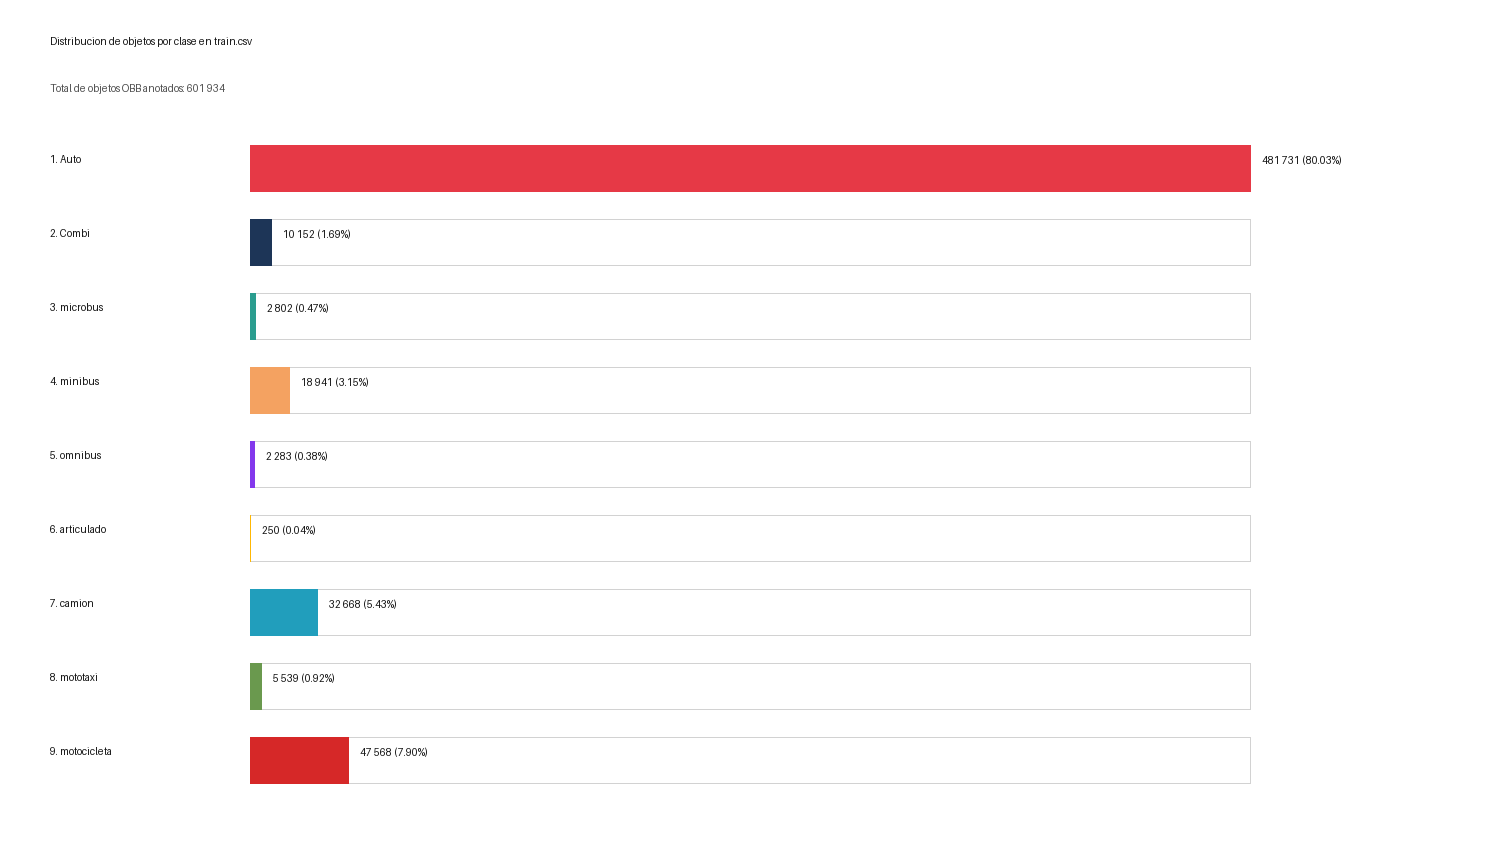
\includegraphics[width=0.95\textwidth]{latex_report/src/fig/dataset_class_distribution.png}
  \caption{Distribuci{\'o}n de objetos anotados por clase vehicular en el conjunto de entrenamiento.}
  \label{fig:dataset_class_distribution}
\end{figure*}

La estructura temporal tambi{\'e}n es importante para el dise{\~n}o experimental. En entrenamiento se identificaron 1 088 clips anonimizados, con un m{\'i}nimo de 18 frames por clip, una media de 49.87, una mediana de 50 y un m{\'a}ximo de 50. En prueba se identificaron 473 clips, con un m{\'i}nimo de 23 frames, media de 49.85, mediana de 50 y m{\'a}ximo de 50. Esta organizaci{\'o}n indica que muchos frames son temporalmente cercanos; por ello, la partici{\'o}n de validaci{\'o}n debe realizarse por clips completos y no por frames individuales, ya que mezclar frames consecutivos del mismo clip entre entrenamiento y validaci{\'o}n podr{\'i}a sobreestimar el rendimiento del modelo.

\begin{figure}[htbp]
  \centering
  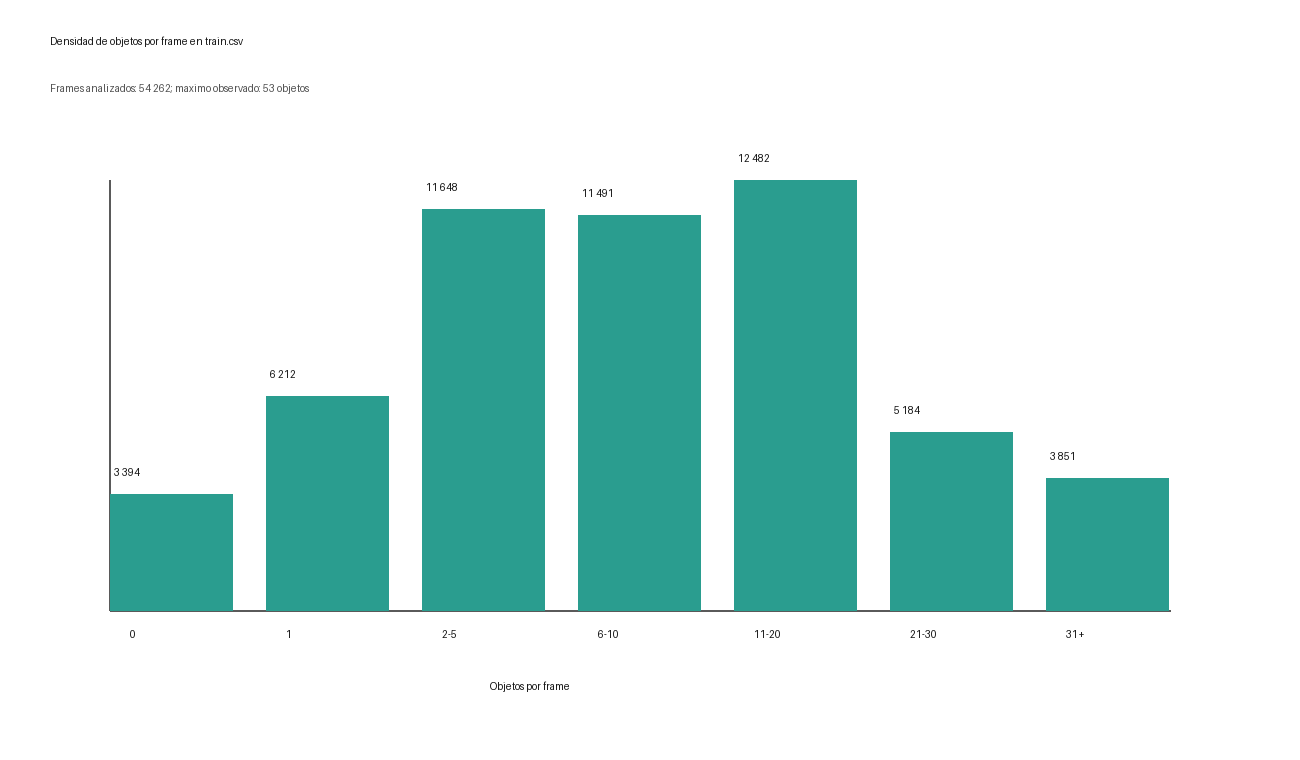
\includegraphics[width=\columnwidth]{latex_report/src/fig/dataset_objects_per_frame.png}
  \caption{Distribuci{\'o}n de densidad de objetos por frame en \texttt{train.csv}.}
  \label{fig:dataset_objects_per_frame}
\end{figure}

La revisi{\'o}n visual confirma que las anotaciones corresponden a cajas orientadas sobre veh{\'i}culos observados desde una perspectiva superior. La Fig.~\ref{fig:dataset_obb_sample} muestra un frame de una intersecci{\'o}n urbana con autos, combi, cami{\'o}n, minibus y motocicleta, donde las cajas siguen la orientaci{\'o}n real de cada veh{\'i}culo. Este ejemplo ilustra por qu{\'e} una representaci{\'o}n horizontal ser{\'i}a insuficiente: algunos veh{\'i}culos aparecen alineados con carriles horizontales, otros con carriles verticales o maniobras de giro, y otros se ubican en zonas de borde o con tama{\~n}os reducidos. En consecuencia, el dataset exige conservar la geometr{\'i}a orientada durante la conversi{\'o}n y el entrenamiento.

\begin{figure*}[htbp]
  \centering
  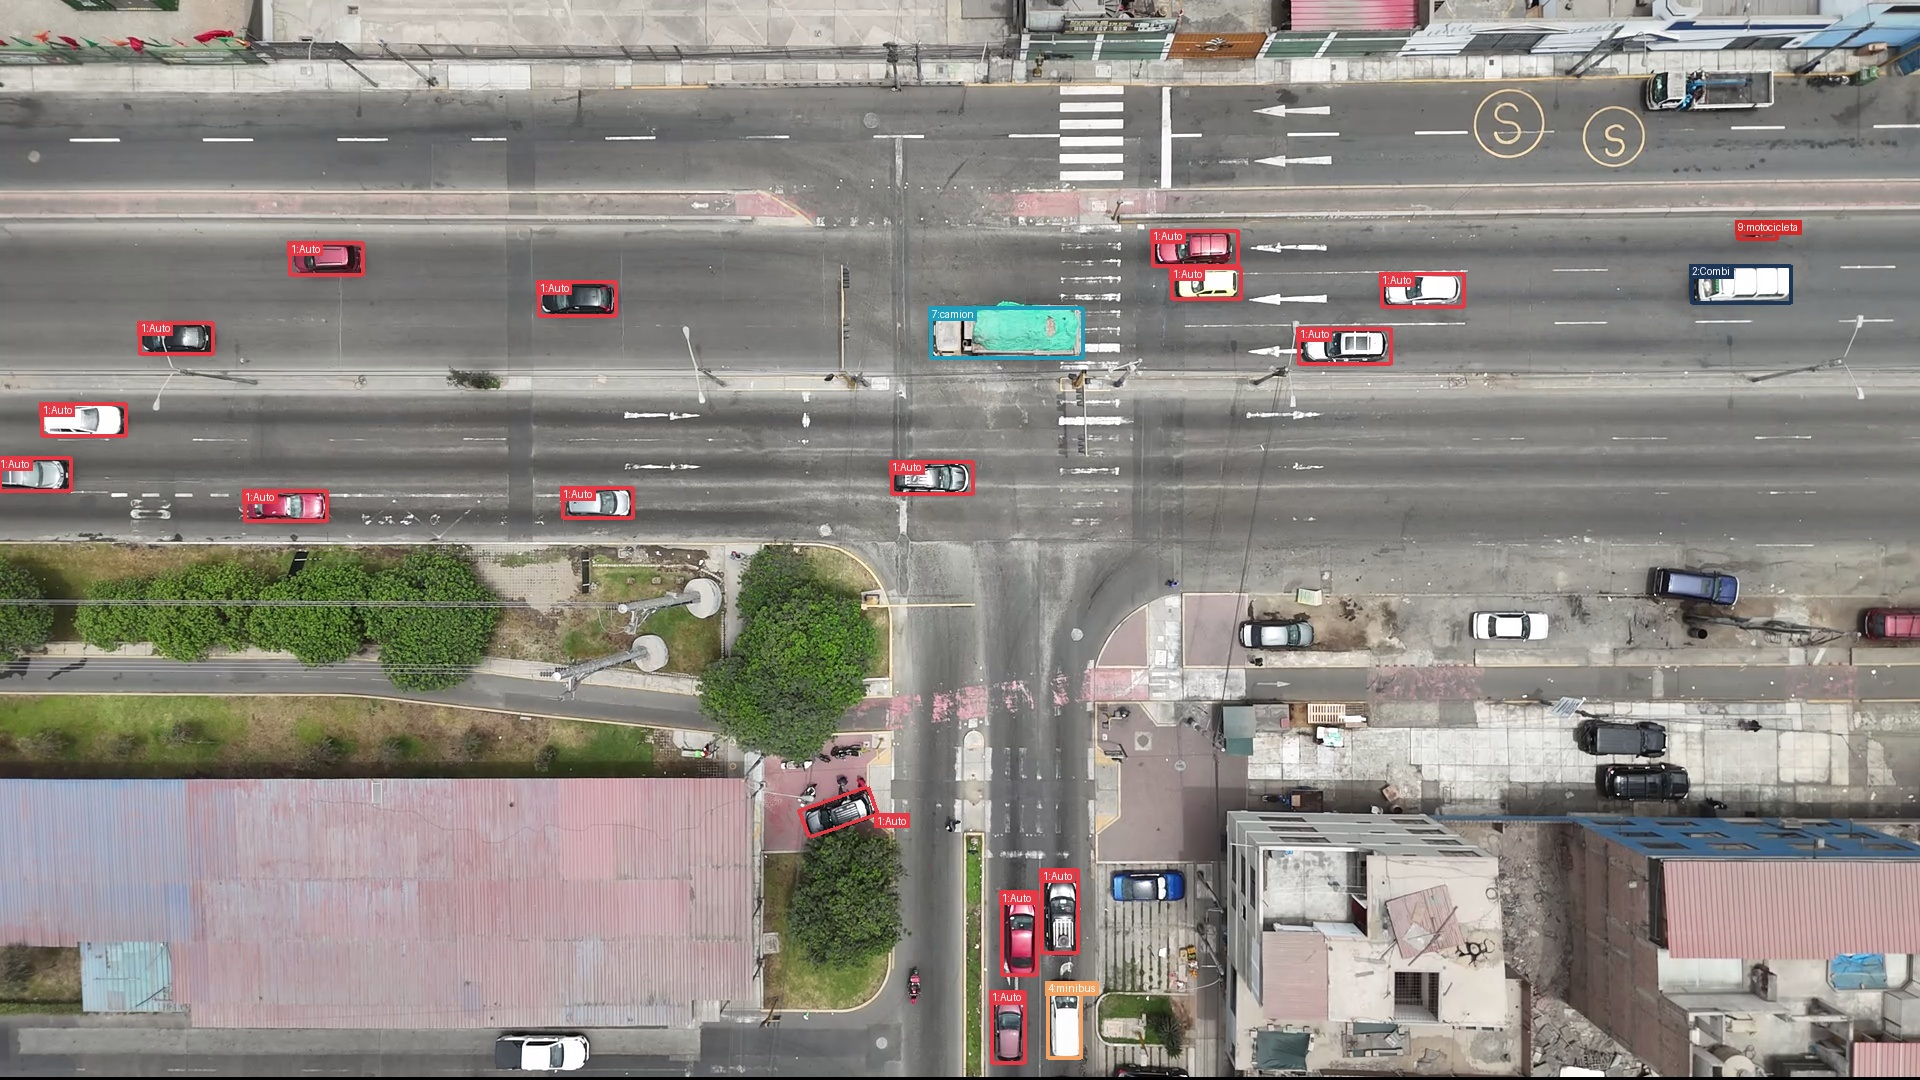
\includegraphics[width=0.95\textwidth]{latex_report/src/fig/dataset_obb_sample.jpg}
  \caption{Ejemplo de frame del conjunto \texttt{muestra\_300/} con anotaciones OBB dibujadas sobre veh{\'i}culos.}
  \label{fig:dataset_obb_sample}
\end{figure*}

En t{\'e}rminos metodol{\'o}gicos, el dataset debe tratarse como un conjunto de frames derivados de clips, no como im{\'a}genes independientes sin relaci{\'o}n temporal. La conversi{\'o}n a un formato compatible con YOLO OBB debe mapear las clases oficiales de 1--9 a clases internas 0--8 y revertir ese mapeo al generar la entrega final. Los frames con \texttt{Target == none} deben mantenerse como im{\'a}genes negativas, porque aportan informaci{\'o}n sobre ausencia de veh{\'i}culos anotados y ayudan a controlar falsos positivos. Finalmente, debido al desbalance de clases y a la evaluaci{\'o}n macro, el an{\'a}lisis del modelo no debe limitarse a la precisi{\'o}n global, sino reportar el comportamiento por clase, especialmente en \texttt{articulado}, \texttt{omnibus}, \texttt{microbus}, \texttt{mototaxi} y \texttt{combi}.

\section{Results and Discussion}
\label{sec:results_discussion}

\subsection{Results}
\label{sec:results}

This section presents the findings of the completed ablation study using the final evaluator artifacts produced for the six experimental conditions: Base 0, Base 1, Base 2, Improvement A, Improvement B, and Improvement C. The final comparison is based on the homogeneous ZIP schema containing \texttt{summary.json}, \texttt{metrics\_by\_class.csv}, \texttt{metrics\_by\_threshold.csv}, \texttt{hardware.json}, raw predictions, filtered predictions, homographies, and manifest metadata.

The final evaluator uses 10,873 validation frames and 109,448 ground-truth vehicle instances. Each model is evaluated with the same inference confidence threshold, class remapping, homography-based motion filter, and Macro AP-rIoU implementation. Figure~\ref{fig:final_evaluation_flow} summarizes this flow because it is central to the interpretation of the results: a detector can emit many candidate boxes and still obtain zero AP if no candidate satisfies the final class and rotated-geometry match.

\begin{figure*}[!t]
  \centering
  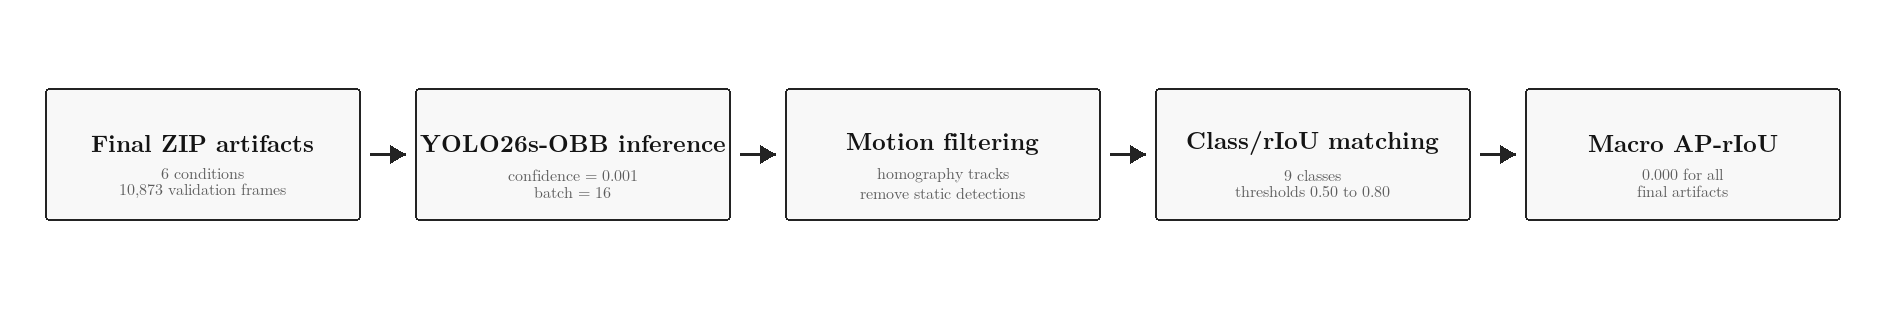
\includegraphics[width=0.93\textwidth]{latex_report/src/fig/final_evaluation_flow.png}
  \caption{Final evaluation flow applied to each ablation artifact. The same validation frames, prediction threshold, motion filter, class mapping, and rIoU thresholds are used for the six conditions.}
  \label{fig:final_evaluation_flow}
\end{figure*}

\subsubsection{Dataset and Augmentation Artifacts}
\label{sec:dataset_characterization_results}

The preprocessing audit confirms that the source training CSV contains 54,262 frames, 1,088 clips, and 601,934 oriented-box annotations. The validation subset used by the final evaluator contains 10,873 frames and 109,448 ground-truth instances, which means that the reported detector results are measured on a fixed validation partition rather than on synthetic or resampled validation data.

The train-only augmentation release, named SAM CP production v1, contains 1,501 synthetic images and 1,501 matching YOLO-OBB label files, with 3,391 inserted vehicle instances. No synthetic validation files are generated. This is important because the ablation is designed to test whether synthetic training evidence helps the model, not whether synthetic examples leak into the validation set. Table~\ref{tab:augmentation_release_summary} summarizes the generated augmentation set.

\begin{table}[!t]
  \caption{SAM copy-paste augmentation set used for training.}
  \label{tab:augmentation_release_summary}
  \centering
  \small
  \begin{tabular}{@{}p{0.60\columnwidth}p{0.32\columnwidth}@{}}
    \toprule
    \textbf{Indicator} & \textbf{Value} \\
    \midrule
    Run ID & SAM CP production v1 \\
    Synthetic images & 1,501 \\
    Synthetic label files & 1,501 \\
    Inserted instances & 3,391 \\
    Validation files generated & 0 \\
    Kernel elapsed time & 652.35 s \\
    Peak GPU memory & 3,297 MiB \\
    Peak GPU utilization & 99\% \\
    \bottomrule
  \end{tabular}
\end{table}

The validation checks cover the main failure modes that could compromise the augmentation release: image-label stem mismatches, empty deltas, malformed YOLO-OBB labels, out-of-range coordinates, synthetic files that shadow real frames, and synthetic backgrounds taken from outside the train split. These checks support the reproducibility of the augmentation process. However, they do not by themselves prove that the generated data improves the detector; that claim must come from the final evaluator.

\subsubsection{Ablation Artifact Status}
\label{sec:ablation_artifact_status}

Table~\ref{tab:ablation_artifact_status} records the final artifact used for each experimental condition. Since every condition is represented by a final evaluator ZIP, the six runs can be compared under the same final metric schema.

\begin{table*}[!t]
  \caption{Final ablation artifacts available for analysis.}
  \label{tab:ablation_artifact_status}
  \centering
  \small
  \begin{tabular}{p{0.14\textwidth} p{0.27\textwidth} p{0.22\textwidth} p{0.27\textwidth}}
    \toprule
    \textbf{Condition} & \textbf{Role in the ablation} & \textbf{Final weight} & \textbf{Artifact interpretation} \\
    \midrule
    Base 0 & Zero-shot YOLO26s-OBB with DOTA vehicle mapping & \texttt{yolo26s-obb.pt} & Final evaluator ZIP; reference without task-specific training \\
    Base 1 & Raw-data baseline with minimal online augmentation & \texttt{f1\_c1\_best.pt} & Final evaluator ZIP; raw trained baseline \\
    Base 2 & Raw-data baseline with stronger classical YOLO augmentation & \texttt{f1\_c2\_best.pt} & Final evaluator ZIP; classical augmentation baseline \\
    Improvement A & LaMa-corrected training pixels with minimal profile & \texttt{f1\_c3\_best.pt} & Final evaluator ZIP; pixel-correction ablation \\
    Improvement B & Raw pixels plus train-only SAM copy-paste delta & \texttt{f1\_mejora\_b\_best.pt} & Final evaluator ZIP plus internal training logs \\
    Improvement C & LaMa-corrected pixels plus the same SAM copy-paste delta & \texttt{f1\_mejora\_c\_best.pt} & Final evaluator ZIP; combined pixel-correction and copy-paste ablation \\
    \bottomrule
  \end{tabular}
\end{table*}

\subsubsection{Final Macro AP-rIoU Comparison}
\label{sec:final_macro_ap_results}

Table~\ref{tab:ablation_final_metrics} and Figure~\ref{fig:ablation_macro_metrics} show the central result of the final artifact set: every condition obtains 0.000 Macro AP-rIoU, 0.000 AP@0.50, and 0.000 AP@0.80. This includes the raw trained baseline, the classical augmentation baseline, the LaMa-only condition, and both SAM copy-paste conditions. The result is therefore not a small performance difference among methods; it is a complete failure to produce accepted true positives under the final class-and-rotated-geometry matcher.

The count snapshot at rIoU 0.50 confirms the same conclusion. The true-positive count is zero for all conditions, while the false-negative count remains 109,448, equal to the number of validation ground-truth instances. Since rIoU 0.50 is the least strict threshold reported in the final metric, the zero result at this threshold implies that the failure is already present before the stricter 0.55--0.80 thresholds are applied.

\begin{table*}[!t]
  \caption{Final ablation metrics. Counts are reported at rIoU 0.50 after motion filtering.}
  \label{tab:ablation_final_metrics}
  \centering
  \scriptsize
  \resizebox{\textwidth}{!}{%
  \begin{tabular}{p{0.14\textwidth} c c c p{0.23\textwidth} c c}
    \toprule
    \textbf{Condition} & \textbf{Macro AP-rIoU} & \textbf{AP@0.50} & \textbf{AP@0.80} & \textbf{TP / FP / FN @0.50} & \textbf{FPS} & \textbf{Mean inference} \\
    \midrule
    Base 0 & 0.000 & 0.000 & 0.000 & 0 / 319,557 / 109,448 & 38.9 & 16.87 ms \\
    Base 1 & 0.000 & 0.000 & 0.000 & 0 / 149,092 / 109,448 & 84.9 & 6.61 ms \\
    Base 2 & 0.000 & 0.000 & 0.000 & 0 / 252,890 / 109,448 & 85.5 & 6.30 ms \\
    Improvement A & 0.000 & 0.000 & 0.000 & 0 / 253,713 / 109,448 & 83.8 & 6.03 ms \\
    Improvement B & 0.000 & 0.000 & 0.000 & 0 / 261,587 / 109,448 & 90.2 & 5.71 ms \\
    Improvement C & 0.000 & 0.000 & 0.000 & 0 / 201,344 / 109,448 & 98.9 & 5.66 ms \\
    \bottomrule
  \end{tabular}
  }
\end{table*}

\begin{figure*}[!t]
  \centering
  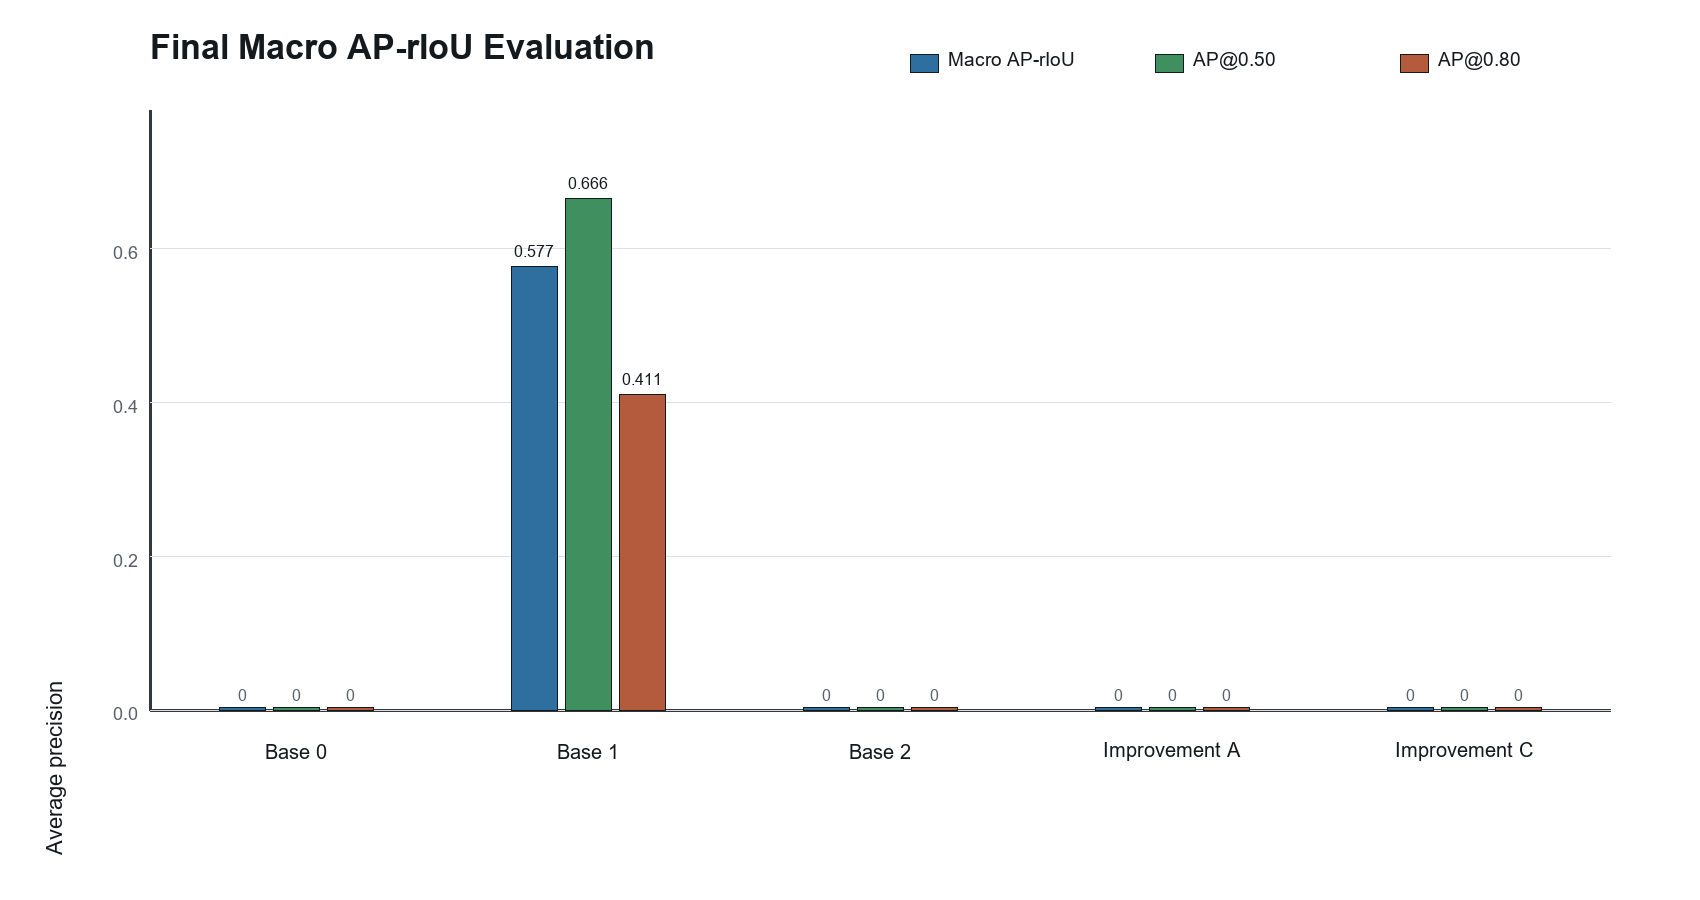
\includegraphics[width=0.90\textwidth]{latex_report/src/fig/ablation_macro_metrics.png}
  \caption{Final Macro AP-rIoU, AP@0.50, and AP@0.80 for the six final evaluator artifacts. All three AP summaries are 0.000 for every condition.}
  \label{fig:ablation_macro_metrics}
\end{figure*}

\begin{figure*}[!t]
  \centering
  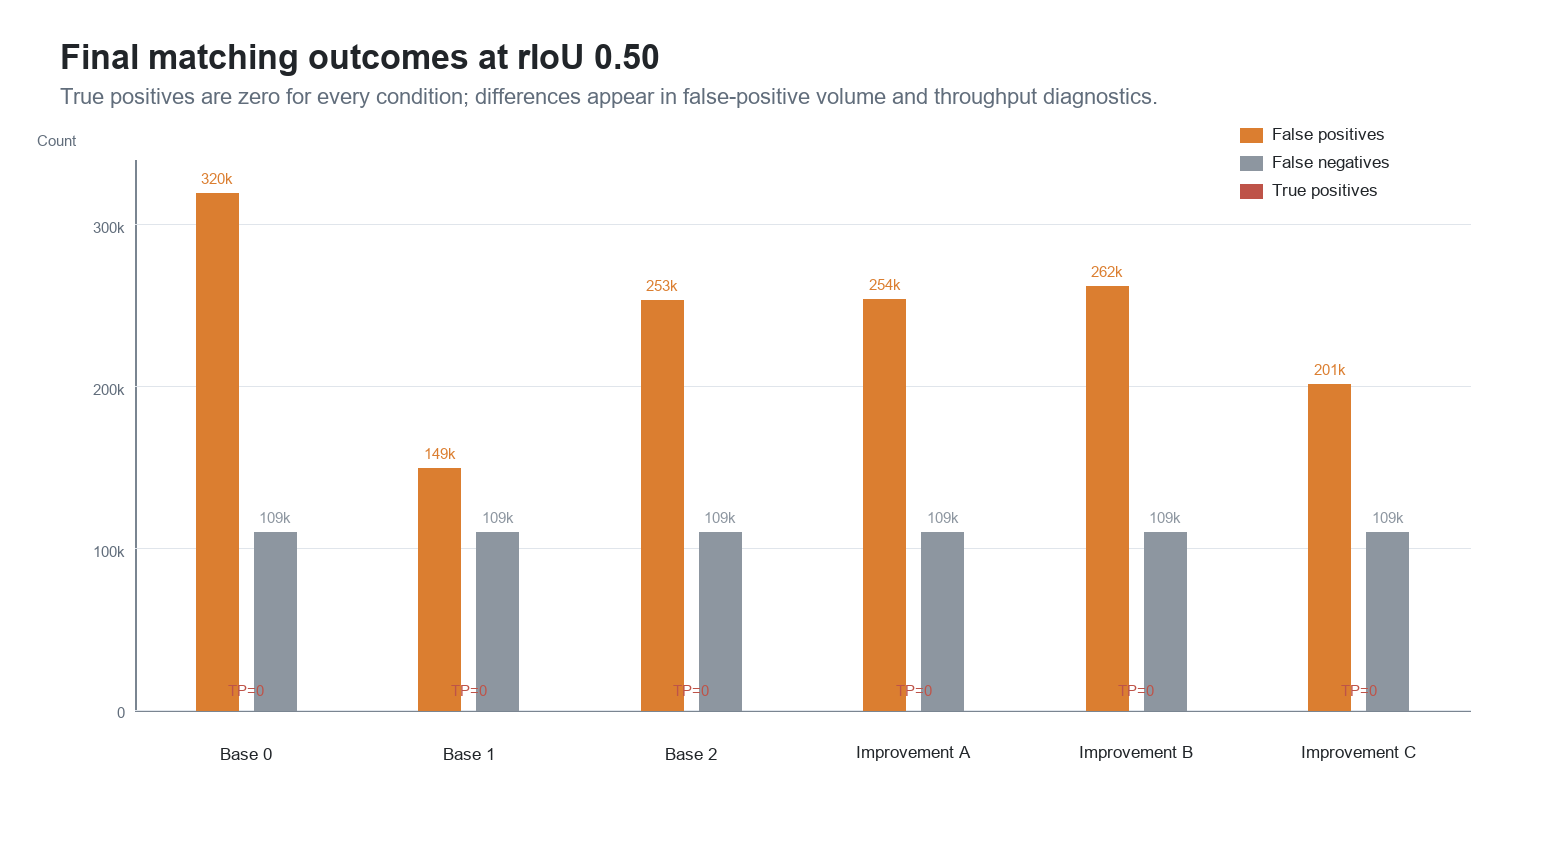
\includegraphics[width=0.92\textwidth]{latex_report/src/fig/ablation_outcomes_riou50.png}
  \caption{True positives, false positives, and false negatives at rIoU 0.50 after motion filtering. Every condition emits candidate detections, but none is accepted as a true positive by the final evaluator.}
  \label{fig:ablation_outcomes_riou50}
\end{figure*}

\subsubsection{Operational and Motion-Filter Diagnostics}
\label{sec:operational_diagnostics_results}

Although all AP values are zero, the artifacts are still informative because they show how each condition behaves before final matching. Figure~\ref{fig:ablation_fp_fps} compares false-positive volume and throughput. Base 0 is the slowest condition and has the highest false-positive count, which is consistent with a zero-shot model using only a partial DOTA-to-task class mapping. Base 1 has the lowest false-positive count among the trained conditions, with 149,092 false positives at rIoU 0.50, but it still has no true positives. Base 2, Improvement A, and Improvement B all increase the post-filter false-positive volume relative to Base 1.

Among the synthetic and LaMa-related variants, Improvement C has the best operational profile. It reduces false positives to 201,344, which is 20.4\% lower than Base 2, 20.7\% lower than Improvement A, and 23.0\% lower than Improvement B. It is also the fastest condition, reaching 98.9 FPS. This suggests that the LaMa plus SAM copy-paste setup changes the detector's candidate distribution in a useful operational direction. However, this cannot be reported as a detection-performance gain because the true-positive count remains zero and the final Macro AP-rIoU remains 0.000.

\begin{figure*}[!t]
  \centering
  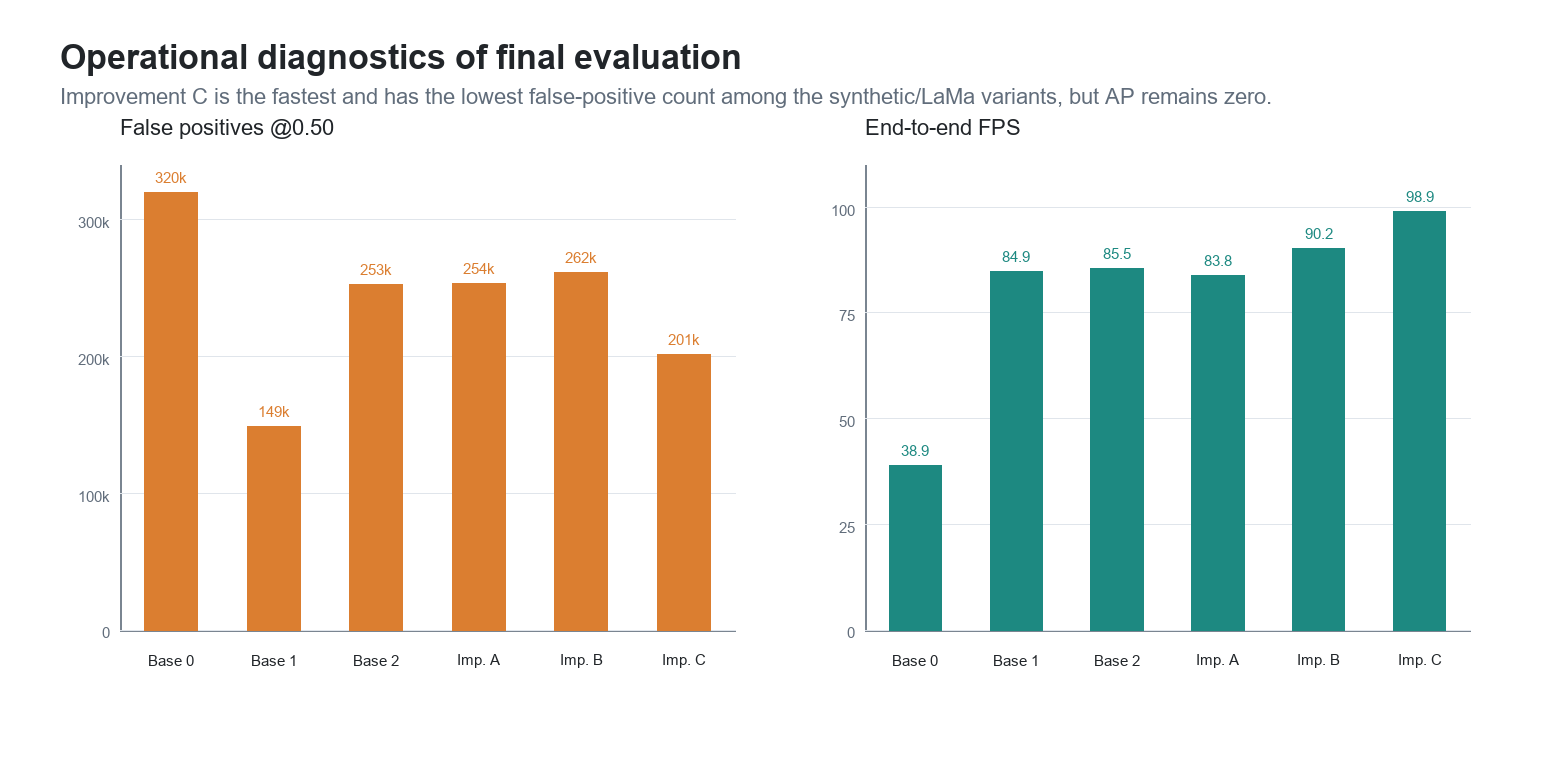
\includegraphics[width=0.92\textwidth]{latex_report/src/fig/ablation_fp_fps.png}
  \caption{Operational comparison of false-positive count and end-to-end throughput. Improvement C reduces false positives among the synthetic/LaMa variants and records the highest FPS, but the final AP score remains zero.}
  \label{fig:ablation_fp_fps}
\end{figure*}

The motion-filter diagnostics in Table~\ref{tab:motion_filter_diagnostics} also show that the evaluator is not simply discarding every prediction. The number of removed predictions varies by condition, from 43,172 in Base 1 to 306,852 in Base 0. The trained conditions form thousands of tracks, and the filter removes a subset identified as static. Therefore, the zero AP result should be interpreted as a final matching problem after filtering rather than as the absence of model output.

\begin{table*}[!t]
  \caption{Motion-filter and runtime diagnostics from the final evaluator artifacts.}
  \label{tab:motion_filter_diagnostics}
  \centering
  \scriptsize
  \resizebox{\textwidth}{!}{%
  \begin{tabular}{p{0.16\textwidth} r r r r r}
    \toprule
    \textbf{Condition} & \textbf{Removed predictions} & \textbf{Static tracks} & \textbf{Total tracks} & \textbf{Elapsed time} & \textbf{FPS} \\
    \midrule
    Base 0 & 306,852 & 9,120 & 56,619 & 279.7 s & 38.9 \\
    Base 1 & 43,172 & 1,539 & 23,385 & 128.1 s & 84.9 \\
    Base 2 & 81,956 & 3,466 & 58,591 & 127.2 s & 85.5 \\
    Improvement A & 100,053 & 3,827 & 51,784 & 129.8 s & 83.8 \\
    Improvement B & 101,569 & 4,122 & 51,392 & 120.6 s & 90.2 \\
    Improvement C & 78,594 & 3,043 & 39,144 & 109.9 s & 98.9 \\
    \bottomrule
  \end{tabular}
  }
\end{table*}

\subsubsection{Class-Level Error Distribution}
\label{sec:class_error_distribution_results}

Because no condition obtains non-zero AP, class-level AP cannot be used to identify strong classes. The useful class-level evidence is instead the distribution of false positives at rIoU 0.50, shown in Figure~\ref{fig:class_fp_by_condition}. Auto dominates the false-positive volume in every trained condition, which is expected because it is the majority class in the dataset. Motocicleta is the second major source of unmatched detections for Base 1, Base 2, Improvement A, and Improvement B. Improvement C reduces Motocicleta false positives to 67,510, compared with 120,836 in Improvement B and 114,589 in Improvement A, but it still does not recover any true positive under the final evaluator.

The heatmap also clarifies the role of Base 0. Its predictions are concentrated in Auto and Camion because the zero-shot DOTA mapping only connects the pretrained vehicle categories to those official task classes. This makes Base 0 useful as a sanity reference for zero-shot inference, but not as a complete nine-class trained model.

\begin{figure*}[!t]
  \centering
  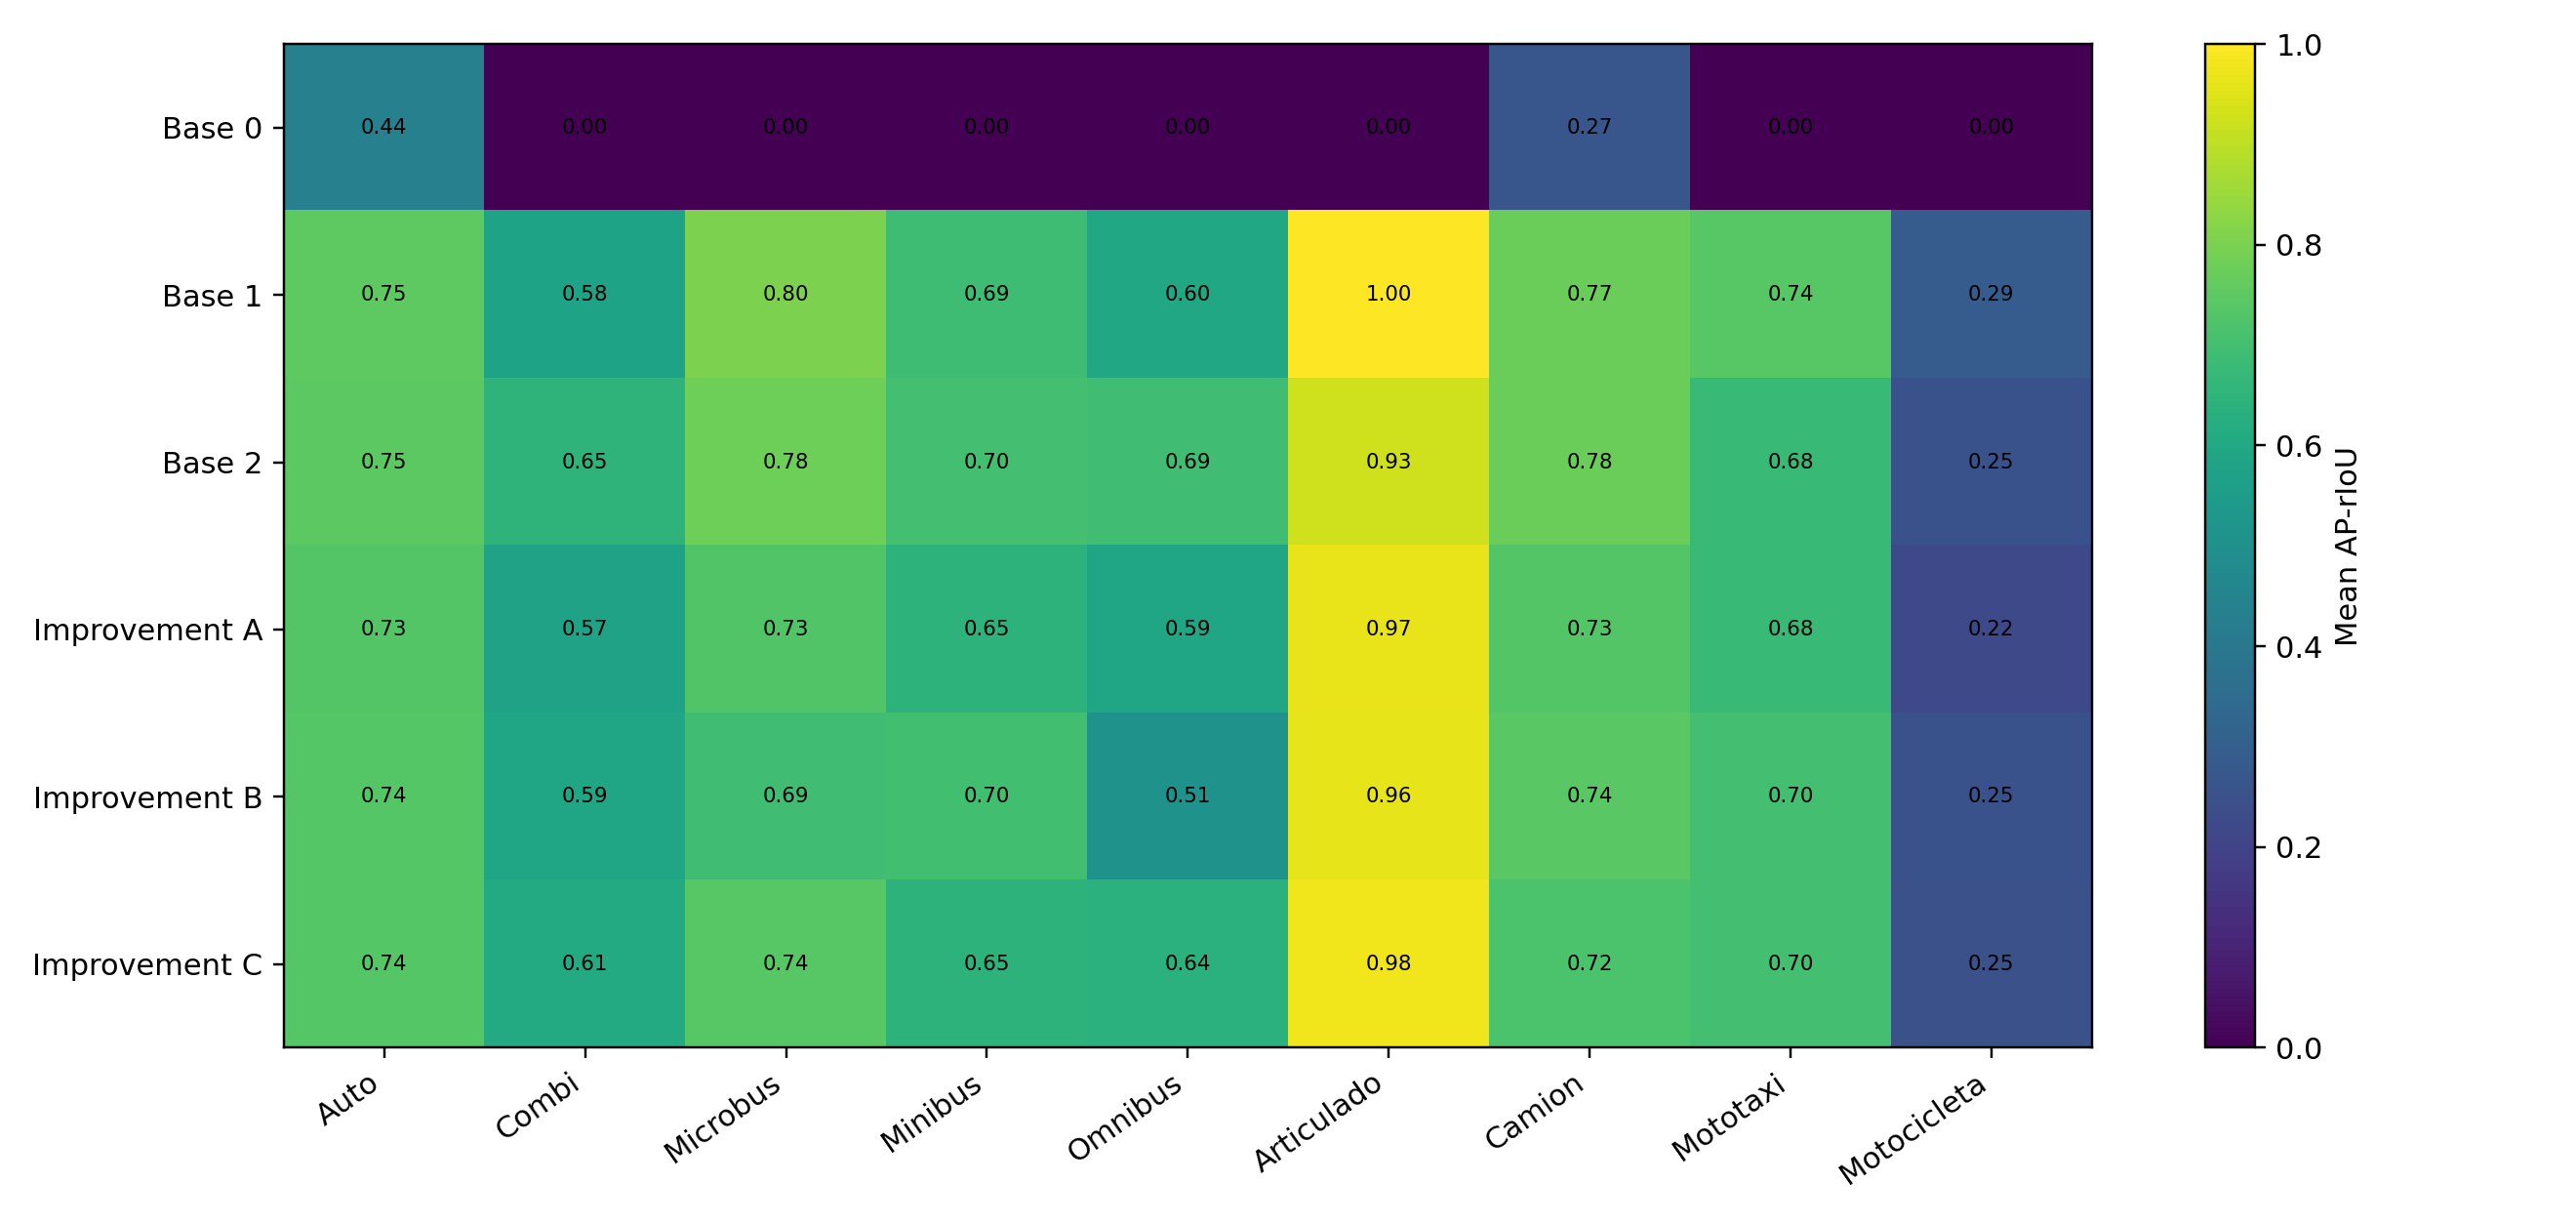
\includegraphics[width=0.95\textwidth]{latex_report/src/fig/class_fp_by_condition.png}
  \caption{False-positive distribution by class at rIoU 0.50. Values are post-filter false positives; color intensity is log-scaled for readability.}
  \label{fig:class_fp_by_condition}
\end{figure*}

\subsubsection{Improvement B Internal Training Evidence}
\label{sec:improvement_b_training_results}

Improvement B now has a final evaluator ZIP, but its training artifacts remain useful because they expose a sharp discrepancy between internal validation and final scoring. The uploaded run completed 12 epochs of a requested 40-epoch schedule with patience 5, batch size 96, image size 640, AdamW, automatic mixed precision, and two Tesla T4 GPUs. The best internal Ultralytics validation mAP50 is 0.929 at epoch 11, and the best internal mAP50-95 is 0.761 at epoch 7. The last recorded epoch reports precision 0.900, recall 0.859, mAP50 0.928, and mAP50-95 0.757.

\begin{figure*}[!t]
  \centering
  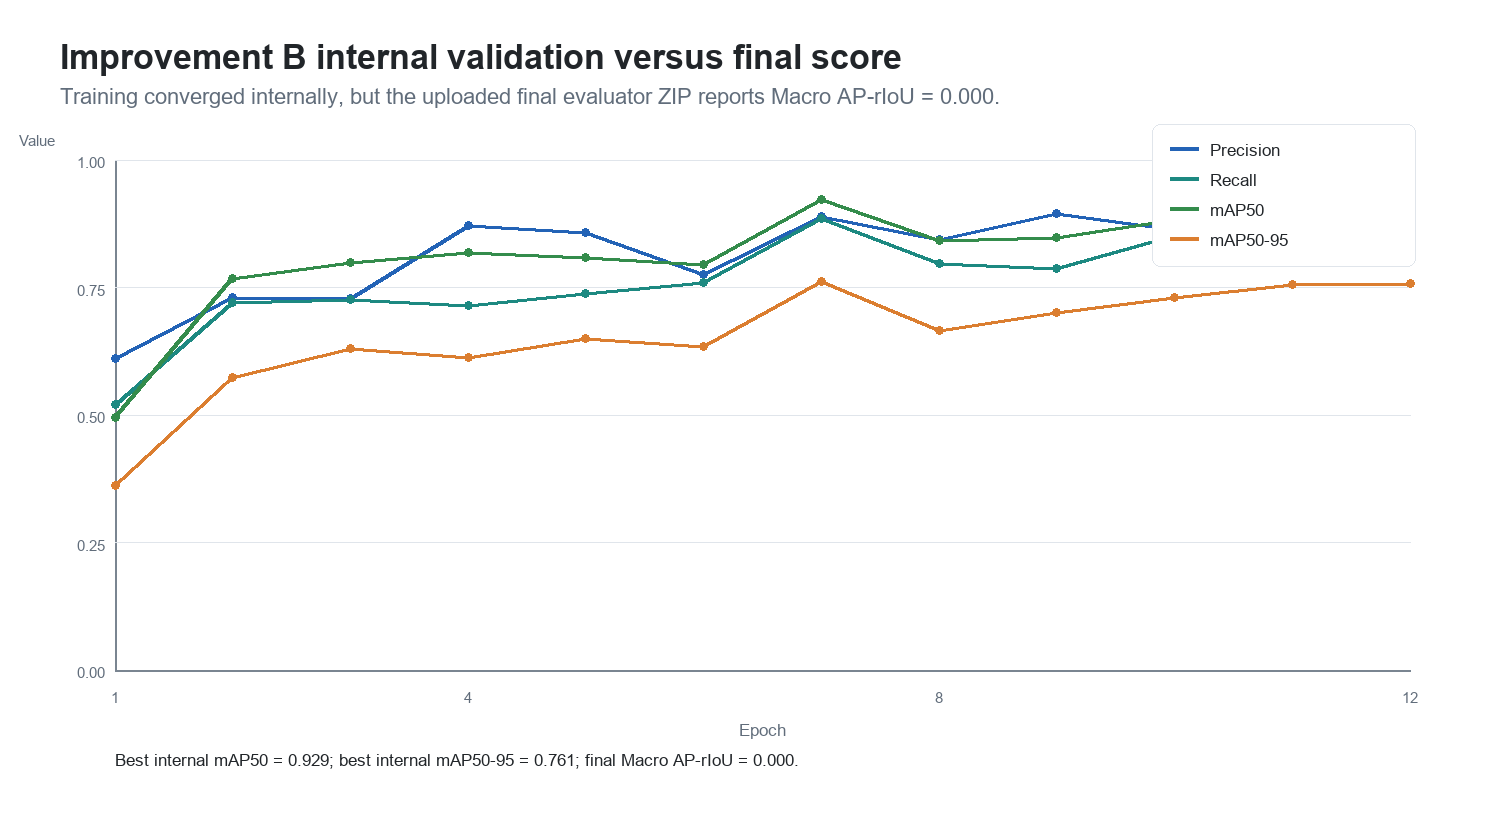
\includegraphics[width=0.90\textwidth]{latex_report/src/fig/mejora_b_training_curves.png}
  \caption{Internal Ultralytics validation curves for Improvement B. The run converges internally, but the final Macro AP-rIoU evaluator reports 0.000 for the same condition.}
  \label{fig:mejora_b_training_curves}
\end{figure*}

This discrepancy is one of the most important diagnostic findings of the study. Ultralytics validation and the paper's final evaluator are not identical measurements: the final score uses the SMART validation frames, official class identifiers, rotated-IoU thresholds, homography-based motion filtering, and the final class-and-geometry matching implementation. Therefore, the high internal mAP of Improvement B cannot be interpreted as evidence of final detector improvement. Instead, it indicates that the next technical priority is to audit the boundary between training validation outputs and final evaluator inputs.

\subsubsection{Summary of Key Findings}
\label{sec:key_findings_results}

Table~\ref{tab:key_findings} summarizes the main findings. The ablation does not support the hypothesis that the current SAM copy-paste release improves final Macro AP-rIoU. It does, however, produce a useful negative result: the augmentation pipeline is reproducible, all final artifacts are now available, and the final evaluator exposes a systematic mismatch that must be resolved before model-quality conclusions can be strengthened.

\begin{table*}[!t]
  \caption{Key findings from the completed final-artifact analysis.}
  \label{tab:key_findings}
  \centering
  \small
  \begin{tabular}{p{0.25\textwidth} p{0.33\textwidth} p{0.34\textwidth}}
    \toprule
    \textbf{Finding} & \textbf{Evidence} & \textbf{Interpretation} \\
    \midrule
    All final AP summaries are zero & Six final evaluator ZIPs report 0.000 Macro AP-rIoU, 0.000 AP@0.50, and 0.000 AP@0.80. & No condition can be claimed as the strongest detector under the current final metric. \\
    Candidate detections are present & False positives range from 149,092 to 319,557 at rIoU 0.50. & The failure occurs at final matching after prediction and filtering, not because models emit no boxes. \\
    Improvement C has the best operational profile among synthetic variants & 201,344 false positives and 98.9 FPS. & It improves candidate volume and speed relative to Base 2, Improvement A, and Improvement B, but not final AP. \\
    Improvement B has a training-final mismatch & Internal mAP50 reaches 0.929, while final Macro AP-rIoU is 0.000. & Training-loop validation is not a substitute for the paper's final evaluator. \\
    The next step is a compatibility audit & Zero true positives appear even at rIoU 0.50. & Class remapping, OBB vertex order, coordinate convention, confidence handling, and motion-filter effects must be checked. \\
    \bottomrule
  \end{tabular}
\end{table*}

\section{Discussion}
\label{sec:discussion}
Discussion goes here.

One-column table example:

\begin{table}[H]
  \centering
  \caption{Table example}
  \label{tab:table2}
  \begin{tabular*}{\hsize}{l p{4cm}}
    \hline
    \textbf{Parameter} & \textbf{Description} \\
    \hline
    Parameter1 & Text of example. \\
    Parameter2 & Text of example. \\
    Parameter3 & Text of example. \\
    Parameter4 & Text of example. \\
    \hline
  \end{tabular*}
\end{table}

\section{Conclusions}
\label{sec:conclusions}

A controlled ablation was conducted to measure segmentation-guided synthetic augmentation for rotated vehicle detection in Peruvian traffic footage. The process included an audit of SMART annotations, conversion to YOLO-OBB labels, preservation of a clip-separated validation set, generation of 1,501 training-only image--label pairs with 3,391 inserted objects, training of YOLO26s-OBB configurations, and uniform evaluation of six artifacts through Macro AP-rIoU and homography-based motion filtering.

Base 1 provides the best aggregate result, with 0.6917 Macro AP-rIoU and 0.7662 AP@0.50. Base 2 is close at 0.6892 and leads at the strictest reported overlap level, with AP@0.80 equal to 0.5417. Improvement C is the strongest proposed alternative, obtaining 0.6682 Macro AP-rIoU while also reaching the highest throughput of 98.93 FPS. Its advantage over Improvements A and B does not extend to either raw-image baseline. The tested SAM-assisted copy-paste strategies therefore offer no accuracy gain over the best conventional training condition in this experiment.

At category level, Motocicleta remains the principal weakness, since every trained run records mean AP-rIoU below 0.30 for that label. The comparison between Base 1 and Base 2 also reveals different error profiles: Base 1 suppresses false detections more effectively and leads the aggregate measure, whereas Base 2 recovers more objects and performs better under strict overlap. These differences reinforce the need to judge augmentation with class-aware rotated metrics and explicit error counts, rather than with generated-sample volume or training-time mAP alone.

The main contribution is an auditable protocol for testing synthetic OBB data without contaminating validation. It shows that the combined proposed configuration may be attractive when processing speed is prioritized, but it is not the most accurate detector. Stronger evidence will require repeated seeds, augmentation targeted at difficult small classes, systematic inspection of detection errors, and comparison against model-level improvements designed specifically for oriented boxes.

\section{Limitations and Future Work}
\label{sec:limitations_future_work}

Each F1 configuration was trained once and assessed on a single fixed split. This design is appropriate for a controlled comparison, but it does not measure variation from initialization, minibatch order, or stochastic transformations. In particular, the 0.0025 Macro AP-rIoU separation between Base 1 and Base 2 is small enough that its ordering could change in repeated experiments. Subsequent work should train several seeds and accompany overall and per-class scores with confidence intervals or bootstrap estimates.

The current evidence also comes from one dataset, one detector family, and one implementation of the final evaluator. Results obtained from these cameras should not be assumed to hold for different cities, viewing angles, rotated detectors, or composition pipelines. Evaluation across cameras and external datasets would clarify whether the synthetic variants improve resilience to distribution shift despite their lower score on the present validation set.

Only one fixed synthetic release was examined. A more complete design should vary the number of inserted objects, class allocation, scale, overlap, placement region, scene compatibility, mask quality, blending procedure, and the ratio between real and generated samples. Because Motocicleta is consistently the hardest category, targeted sampling of realistic small-object examples is a priority, provided that scene density and contextual plausibility are preserved. Additional experiments should isolate LaMa correction, SAM-based extraction, placement constraints, and sampling ratio instead of changing several factors simultaneously.

Aggregate AP does not fully explain the observed rankings. Further analysis should include precision--recall curves, category confusions, duplicate predictions, localization failures, and stratification by object size, camera, lighting, congestion, and occlusion. Visual review of matched and unmatched oriented boxes could reveal why Base 1 limits false positives and why Base 2 performs better at rIoU 0.80.

Finally, data modification should be tested alongside changes to the detector itself. Promising comparisons include class-balanced objectives, rare-class resampling, larger input resolution, losses tailored to oriented boxes, hard-example mining, and alternative rotated-detection architectures. Deployment experiments should additionally report latency, memory, and energy use on the intended platform. Such measurements are necessary to determine whether the 98.93 FPS achieved by Improvement C justifies its lower accuracy in a real surveillance system.

\section*{CRediT authorship contribution statement}
\label{sec:authorship_contribution}
CRediT authorship contribution statement goes here.

\section*{Declaration of competing interest}
\label{sec:competing_interest}
The authors declare that they have no known competing financial interests or personal relationships that could have appeared to influence the reported work.

\section*{Ethical statement}
\label{sec:ethical_statement}
The experiments do not involve humans or animals, and no ethical approval was required. An ethical statement is not applicable.

\section*{Consent to participate}
\label{sec:consent_participate}
Not Applicable.

\section*{Consent for publication}
\label{sec:consent_publication}
Not Applicable.

\section*{Funding}
\label{sec:funding}
Not Applicable.

\section*{Acknowledgement}
\label{sec:acknowledgement}
Not Applicable.

\section*{Code availability}
\label{sec:code_availability}
The source code and LaTeX manuscript are available in the \href{https://github.com/unsa-semester-2026-A/ia_article}{public project repository}. The experimental Python package metadata declares an MIT license.

\section*{Data availability}
\label{sec:data_availability}
The data supporting this study's findings are available in (Kaggle) at url: \url{https://www.google.com.pe}.



%% References with BibTeX database:

\bibliographystyle{latex_report/style/elsarticle-num}
\bibliography{latex_report/references}

\end{document}
